% ## http://journals.plos.org/ploscompbiol/s/submit-now
% Template for PLoS
% Version 3.2 March 2016
%
% % % % % % % % % % % % % % % % % % % % % %
%
% -- IMPORTANT NOTE
%
% This template contains comments intended 
% to minimize problems and delays during our production 
% process. Please follow the template instructions
% whenever possible.
%
% % % % % % % % % % % % % % % % % % % % % % % 
%
% Once your paper is accepted for publication, 
% PLEASE REMOVE ALL TRACKED CHANGES in this file 
% and leave only the final text of your manuscript. 
% PLOS recommends the use of latexdiff to track changes during review, as this will help to maintain a clean tex file.
% Visit https://www.ctan.org/pkg/latexdiff?lang=en for info or contact us at latex@plos.org.
%
%
% There are no restrictions on package use within the LaTeX files except that 
% no packages listed in the template may be deleted.
%
% Please do not include colors or graphics in the text.
%
% The manuscript LaTeX source should be contained within a single file (do not use \input, \externaldocument, or similar commands).
%
% % % % % % % % % % % % % % % % % % % % % % %
%
% -- FIGURES AND TABLES
%
% Please include tables/figure captions directly after the paragraph where they are first cited in the text.
%
% DO NOT INCLUDE GRAPHICS IN YOUR MANUSCRIPT
% - Figures should be uploaded separately from your manuscript file. 
% - Figures generated using LaTeX should be extracted and removed from the PDF before submission. 
% - Figures containing multiple panels/subfigures must be combined into one image file before submission.
% For figure citations, please use "Fig" instead of "Figure".
% See http://journals.plos.org/plosone/s/figures for PLOS figure guidelines.
%
% Tables should be cell-based and may not contain:
% - tabs/spacing/line breaks within cells to alter layout or alignment
% - vertically-merged cells (no tabular environments within tabular environments, do not use \multirow)
% - colors, shading, or graphic objects
% See http://journals.plos.org/plosone/s/tables for table guidelines.
%
% For tables that exceed the width of the text column, use the adjustwidth environment as illustrated in the example table in text below.
%
% % % % % % % % % % % % % % % % % % % % % % % %
%
% -- EQUATIONS, MATH SYMBOLS, SUBSCRIPTS, AND SUPERSCRIPTS
%
% IMPORTANT
% Below are a few tips to help format your equations and other special characters according to our specifications. For more tips to help reduce the possibility of formatting errors during conversion, please see our LaTeX guidelines at http://journals.plos.org/plosone/s/latex
%
% For inline equations, please be sure to include all portions of an equation in the math environment.  For example, x$^2$ is incorrect; this should be formatted as $x^2$ (or $\mathrm{x}^2$ if the romanized font is desired).
%
% Do not include text that is not math in the math environment. For example, CO2 should be written as CO\textsubscript{2} instead of CO$_2$.
%
% Please add line breaks to long display equations when possible in order to fit size of the column. 
%
% For inline equations, please do not include punctuation (commas, etc) within the math environment unless this is part of the equation.
%
% When adding superscript or subscripts outside of brackets/braces, please group using {}.  For example, change "[U(D,E,\gamma)]^2" to "{[U(D,E,\gamma)]}^2". 
%
% Do not use \cal for caligraphic font.  Instead, use \mathcal{}
%
% % % % % % % % % % % % % % % % % % % % % % % % 
%
% Please contact latex@plos.org with any questions.
%
% % % % % % % % % % % % % % % % % % % % % % % %

\documentclass[10pt,letterpaper]{article}
\usepackage[top=0.85in,left=2.75in,footskip=0.75in]{geometry}

% Use adjustwidth environment to exceed column width (see example table in text)
\usepackage{changepage}

% Use Unicode characters when possible
\usepackage[utf8x]{inputenc}

% textcomp package and marvosym package for additional characters
\usepackage{textcomp,marvosym}

% fixltx2e package for \textsubscript
\usepackage{fixltx2e}

% amsmath and amssymb packages, useful for mathematical formulas and symbols
\usepackage{amsmath,amssymb}

% cite package, to clean up citations in the main text. Do not remove.
\usepackage{cite}

% Use nameref to cite supporting information files (see Supporting Information section for more info)
\usepackage{nameref,hyperref}

% line numbers
\usepackage[right]{lineno}

% ligatures disabled
\usepackage{microtype}
\DisableLigatures[f]{encoding = *, family = * }

% Remove comment for double spacing
\usepackage{setspace} 
\doublespacing

% Text layout
\raggedright
\setlength{\parindent}{0.5cm}
\textwidth 5.25in 
\textheight 8.75in

% Bold the 'Figure #' in the caption and separate it from the title/caption with a period
% Captions will be left justified
\usepackage[aboveskip=1pt,labelfont=bf,labelsep=period,justification=raggedright,singlelinecheck=off]{caption}
\renewcommand{\figurename}{Fig}

% Use the PLoS provided BiBTeX style
\bibliographystyle{plos2015}

% Remove brackets from numbering in List of References
\makeatletter
\renewcommand{\@biblabel}[1]{\quad#1.}
\makeatother

% Leave date blank
\date{}

% Header and Footer with logo
\usepackage{lastpage,fancyhdr,graphicx}
\usepackage{epstopdf}
\pagestyle{myheadings}
\pagestyle{fancy}
\fancyhf{}
\setlength{\headheight}{27.023pt}
\lhead{
\includegraphics[width=2.0in]{PLOS-submission.eps}}
\rfoot{\thepage/\pageref{LastPage}}
\renewcommand{\footrule}{\hrule height 2pt \vspace{2mm}}
\fancyheadoffset[L]{2.25in}
\fancyfootoffset[L]{2.25in}
\lfoot{\sf PLOS}

%% Include all macros below
\newcommand{\khalf}{\left(\frac{1}{2}\right)^{\delta_{ij}}}  % (1/2)^kronecker
\newcommand{\kkhalf}{\left(\frac{1}{2}\right)^{\delta_{ij} \delta_{kl}}}  % (1/2)^(kronecker * kronecker)
\newcommand{\Lspvl}{$\log_{10}$ SPVL}
\newcommand{\rzero}{{\mathcal R}_0}
\newcommand{\etal}{\textit{et al.}}
\newcommand{\tsub}[2]{#1_{{\textrm{\tiny #2}}}}
\newcommand{\PF}{\textrm{PF}}
\newcommand{\DS}{\textrm{DS}}
\newcommand{\WT}{\textrm{WT}}
\newcommand{\ET}{\textrm{ET}}
\newcommand{\DM}{\textrm{DM}}

%% END MACROS SECTION


\begin{document}
\vspace*{0.2in}

% Title must be 250 characters or less.
\begin{flushleft}
{\Large
\textbf\newline{Effects of Epidemiological Structure on the Transient Evolution of HIV Virulence} % Please use "title case" (capitalize all terms in the title except conjunctions, prepositions, and articles).
}
%% short title: Epidemiological Structure and HIV Virulence Evolution
%% (53/70 characters)
\newline
% Insert author names, affiliations and corresponding author email (do not include titles, positions, or degrees).
\\
Sang Woo Park\textsuperscript{1}
Benjamin M. Bolker\textsuperscript{1,2,3,*}
\\
\bigskip
\textbf{1} Department of Mathematics \& Statistics,  McMaster University, Hamilton, Ontario, Canada
\\
\textbf{2} Department of Biology,  McMaster University, Hamilton, Ontario, Canada
\\
\textbf{3} Institute for Infectious Disease Research,  McMaster University, Hamilton, Ontario, Canada
\\
\bigskip

% Insert additional author notes using the symbols described below. Insert symbol callouts after author names as necessary.
% 
% Remove or comment out the author notes below if they aren't used.
%
% Primary Equal Contribution Note
%\Yinyang These authors contributed equally to this work.

% Additional Equal Contribution Note
% Also use this double-dagger symbol for special authorship notes, such as senior authorship.
%\ddag These authors also contributed equally to this work.

% Current address notes
%\textcurrency Current Address: Dept/Program/Center, Institution Name, City, State, Country % change symbol to "\textcurrency a" if more than one current address note
% \textcurrency b Insert second current address 
% \textcurrency c Insert third current address

% Deceased author note
%\dag Deceased

% Group/Consortium Author Note
%\textpilcrow Membership list can be found in the Acknowledgments section.

% Use the asterisk to denote corresponding authorship and provide email address in note below.
* bolker@mcmaster.ca

\end{flushleft}
% Please keep the abstract below 300 words
% current is 298!
\section*{Abstract}
The evolutionary dynamics of parasite virulence over the
  course of an emerging epidemic have important implications both for
  our basic understanding of epidemiological dynamics and,
  potentially, for the outcomes of public health interventions.
  Changes in the fitness landscape
  will generally select for higher virulence during the early
  phase of an epidemic, but quantitative outcomes
  can depend sensitively on biological details and the structure of
  mathematical models used to capture them.  Fraser, Shirreff, and
  co-workers have proposed a series of models for eco-evolutionary
  dynamics of HIV that are relatively detailed in their portrayal of
  the tradeoffs between transmission and virulence (mediated by
  set-point viral load, SPVL) and their heritability between
  hosts. However, these models use implicit
  representations of the transmission process that drastically simplify the
  partnership dynamics that previous research has found to be critical
  in driving epidemics of sexually transmitted diseases.  We
  explore models that combine HIV virulence tradeoffs with a range of
  epidemiological structures, modeling partnership formation and
  dissolution and allowing for individuals to transmit disease outside
  of partnerships. We assess summary statistics such as the peak value
  of virulence (SPVL) and the time at which the peak occurs across all
  models and across a Latin hypercube sample that captures a realistic
  range of partnership dynamic parameters for sub-Saharan Africa. In
  order to account for the different interpretations of parameters
  across model structures, we scale all parameter sets to constrain
  the simulated epidemic growth rate to be identical, matching a
  realistic baseline value. For this
  particular model setting, the simplest random-mixing structure is
  actually the best approximation to the most realistic model; this
  surprising outcome occurs because the dominance of extra-pair
  contact in the realistic model tends to mask the effects of
  partnership structure.

% Please keep the Author Summary between 150 and 200 words
% Use first person. PLOS ONE authors please skip this step. 
% Author Summary not valid for PLOS ONE submissions.   
\section*{Author Summary}

%% 162 words

Pathogens such as HIV can evolve rapidly in response to changes
in their environments; such changes include both increases in disease
prevalence over the course of the epidemic and treatment
interventions. While researchers have successfully used computational
models to explore these evolutionary dynamics, these models often
neglect details such as the formation and
dissolution of sexual partnerships; other research has shown that
these processes can strongly affect epidemic outcomes. We built and
compared models that used different methods to
model both partnership dynamics and sexual
contact outside of partnerships. Models of intermediate
complexity predicted much lower peak virulence (15 years to
progress to AIDS) compared to both more realistic models
and simple random-mixing models with no partnership structure
at all (both approx. 7.25 years to progress to AIDS); 
extra-pair contact tended to wash out the effects
of epidemiological structure. The large differences
in evolutionary dynamics among different epidemiological models
suggests that researchers trying to predict the evolution of
pathogens should proceed with caution.

\linenumbers

% Use "Eq" instead of "Equation" for equation citations.
\section*{Introduction}

The evolution of pathogen virulence is a fundamental process in
evolutionary biology, of both theoretical and (potentially) practical
importance. The trade-off theory \cite{Ebert1999} --- which
postulates that parasite virulence can be explained as the long-term
evolutionary outcome of a saturating relationship between parasite
clearance rate and transmission rate --- has been criticized
\cite{EbertBull2003,alizon_adaptive_2015}, but has also been
successfully applied in a variety of host-pathogen systems \cite{Dwyer+1990,mackinnon1999genetic,jensen2006empirical,deroode2008virulence}. One
particularly interesting application of these ideas is the work by
Fraser \etal\ showing that HIV appears to satisfy the prerequisites of
the tradeoff theory: in studies of discordant couples (i.e. long-term
sexual partnerships with one infected and one uninfected partner), HIV
virulence as measured by the rate of progression to AIDS was both
heritable and covaried with the set-point viral load (i.e., the
characteristic virus load measured in blood during the intermediate
stage of infection), which in turn predicted the probability of
transmission
\cite{Fraser+2007,fraser_virulence_2014}. Subsequent studies
\cite{shirreff_transmission_2011,herbeck_hiv_2014} used these data to
parameterize mechanistic models of HIV virulence evolution, suggesting
that HIV invading a novel population would initially evolve increased
virulence, peaking after approximately 100-200 years and then declining
slightly to a long-stable virulence level.

The work of Shirreff \etal\ \cite{shirreff_transmission_2011}, and particularly the predicted
transient peak in HIV virulence midway through the epidemic,
highlights the importance of interactions between epidemiological and
evolutionary factors \cite{day_virulence_2004,alizon_price_2009}.
However, despite these studies' attention to detail at the individual
or physiological level, the epidemiological structures used in these
models are relatively simple.

As we discuss in detail below, the
existing models of HIV eco-evolutionary dynamics either use implicit
models that incorporate the average effects of within-couple sexual
contact --- without representing the explicit dynamics of pair
formation and dissolution or accounting for extra-partnership contact
--- or use an agent-based formulation with parameters that effectively
lead to random mixing among infected and uninfected individuals. Here
we explore the effects of incorporating \emph{explicit}
epidemiological structure in eco-evolutionary models.

We add complexity to the epidemiological model following the general approach of Champredon \etal\ \cite{champredon_hiv_2013}; individuals join and leave partnerships at a specified rate, and can have sexual contact both within and outside of established partnerships. In order to explore how virulence evolution depends on epidemiological structure, we consider a series of models with increasing levels of complexity. In order to avoid dependence of the results on a particular set of parameters --- as we explain below, finding matching sets of parameters across models with widely differing epidemiological structures is challenging --- we evaluate our models across a wide range of parameters, again following Champredon \etal\ \cite{champredon_hiv_2013} in using a Latin hypercube design. For each model run, we compute a set of metrics (peak virulence, timing of virulence peak, equilibrium virulence) that summarize the evolutionary trajectory of a simulated HIV epidemic.

As our primary goal is to explore how different epidemiological structures (i.e. partnership dynamics and contact structures) affect our conclusions about the evolution of virulence, our models use a simplified description of within-host dynamics and heritability derived from 
Shirreff \etal's multi-strain evolutionary model \cite{shirreff_transmission_2011}. Like Shirreff \etal, we use a simple susceptible-infected-susceptible demographic formulation; rather than modeling birth and death (or more specifically, recruitment into the sexually active population and death), we assume that whenever an individual dies from infection, another enters the susceptible compartment.

\section*{Materials and Methods}

\subsection*{Infection dynamics}

Like Shirreff \etal\ \cite{shirreff_transmission_2011}, we focus on the evolution of mean $\log_{10}$ set-point viral load, SPVL (which we denote as $\alpha$), rather than the rate of progression to AIDS itself
(we refer to SPVL as ``virulence'' hereafter).
In contrast to Shirreff \etal, we use a single-stage disease model instead of accounting explicitly for progression through the three main stages of HIV infection (primary, asymptomatic, and disease), and we use a simple exponentially distributed infectious period instead of a more realistic Weibull-distributed infectious period. We account for varying transmission rates and durations of each disease stage by summing the durations of three stages (again based on Shirreff \etal's model) and taking the duration-weighted average of transmission rates of three stages. Thus the within-couple transmission rate, $\beta$, for our models is given by:
\begin{equation}
\beta (\alpha) = \frac{D_P \beta_P + D_A (\alpha) \beta_A (\alpha) + D_D \beta_D}{D_P + D_A (\alpha) + D_D},
\end{equation}
where the duration of infection ($D_P$ and $D_D$) and rate of transmission ($\beta_P$ and $\beta_D$) of the Primary and Disease stages
of infection are independent of the host's SPVL. Following Shirreff \etal, the duration of infection ($D_A$) and rate of transmission ($\beta_A$) for the Asymptomatic stage are Hill functions of the SPVL:

\begin{equation}
\begin{split}
D_A(\alpha) &= \frac{\tsub{D}{max} D_{50} ^{D_k}}{V_\alpha ^{D_k} + D_{50}^{D_k}}, \\
\beta_A(\alpha) &= \frac{\tsub{\beta}{max} V_\alpha ^ {\beta_k}}%
{V_\alpha^{\beta_k} + \beta_{50} ^{\beta_k}},
\end{split}
\end{equation}
where $V_{\alpha} = 10^\alpha$. 
The uncoupled and extra-couple transmission rates are scaled by multiplying the within-couple transmission rate $\beta$ by the contact ratios $c_u/c_w$ and $c_e/c_w$.

Although such simplification affects evolution of virulence, we show that our simplified model is able to produce result that is qualitatively similar to that of Shirreff \etal\'s \cite{shirreff_transmission_2011}. 

\subsection*{Mutation}

Like Shirreff \etal\ \cite{shirreff_transmission_2011} we incorporate a between-host mutation process in the SPVL, but simplify Shirreff \etal's evolutionary model by using a one-to-one genotype-phenotype mapping.
The mutational process in our model is directly taken from Shirreff \etal. Over the course of infection, mutation occurs within the host. However, it is assumed that SPVL of an infected individual is determined by the SPVL at the time of infection (and is not further affected by within-host mutation). Instead, the mutational effect takes place when an infected individual transmits the virus to a susceptible individual. First, the distribution of \Lspvl\ is discretized into a vector:
\begin{equation}
\alpha_i = \tsub{\alpha}{min} + (\tsub{\alpha}{max} - \tsub{\alpha}{min})\frac{i-1}{n-1} \qquad i = 1,2,3, \dots n.
\end{equation}
We have experimented with varying degrees of discretization in the strain distribution (i.e., values of $n$); in our model runs comparing results with Shirreff \etal\ \cite{shirreff_transmission_2011} (\figurename~\ref{fig:panel3}) we use $n=51$ (i.e. a bin width of 0.1 \Lspvl\ for $\alpha$), but we find only small differences when reducing $n$ to 21 (bin width = 0.25 \Lspvl), which we use for all other simulations.

\begin{figure}[!ht]
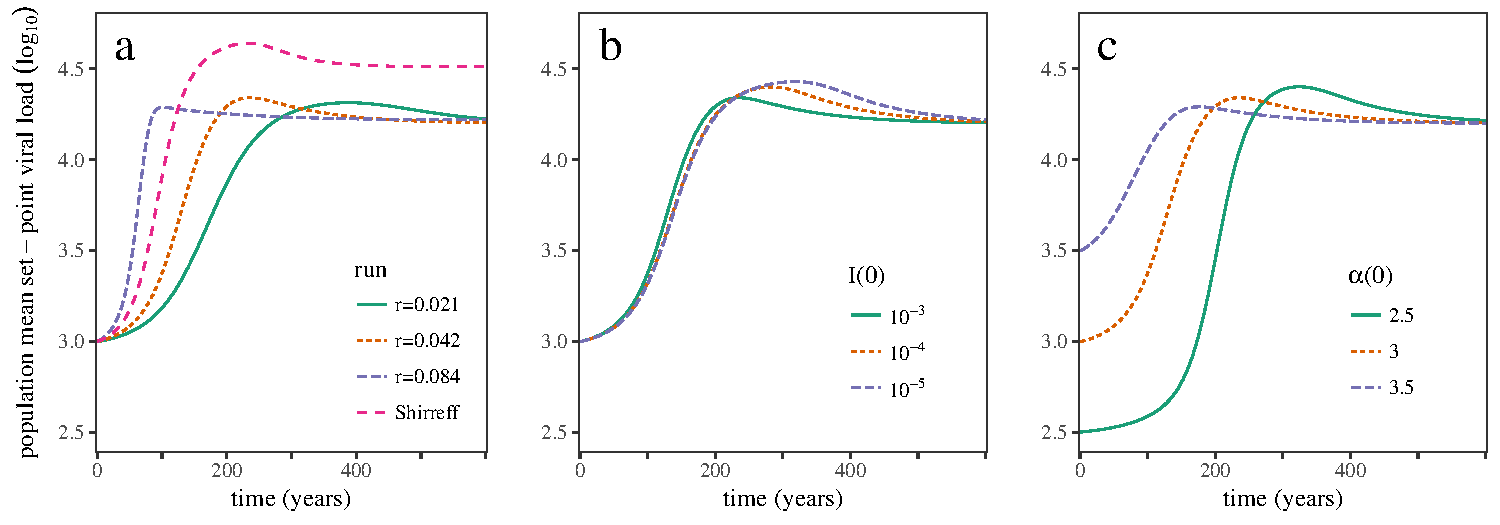
\includegraphics[width=\textwidth]{../figures/fig1.pdf}
\caption{{\bf Baseline dynamics.}
Time series of mean population virulence (\Lspvl). (a) Shirreff model, effects of varying $r$. (b) Effects of varying initial infectious density $I(0)$. (c) Effects of varying initial mean virulence $\alpha(0)$.}
\label{fig:panel3}
\end{figure}

We construct an $n$ by $n$ mutational matrix, $M$ --- which is multiplied with the transmission term ---  so that $M_{ij}$ is the probability that a newly infected individual will have \Lspvl\ of $\alpha_j$ given that the infector has \Lspvl\ of $\alpha_i$. Finally, the probabilities are normalized so that each row sums to 1:
\begin{equation}
M_{ij} = \frac{\Phi(\alpha_j + d/2;i) - \Phi(\alpha_j - d/2;i)}{\Phi(\tsub{\alpha}{max} + d/2;i) - \Phi(\tsub{\alpha}{min} - d/2;i)},
\end{equation}
where $\Phi(x;i)$ is the Gaussian cumulative distribution function with mean $\alpha_i$ and variance of $\sigma_M^2$, and $d = (\tsub{\alpha}{max} - \tsub{\alpha}{min})/(n-1)$. Transmission rate and disease induced mortality rates are discretized into a vector as well:
\begin{equation}
\begin{aligned}
\beta_i &= \beta(\alpha_i),\\
\lambda_i &= \frac{1}{D_P + D_A (\alpha_i) + D_D}.
\end{aligned}
\end{equation}

\subsection*{Contact structure and partnership dynamics}

We developed seven multi-strain evolutionary models covering a gamut between Champredon \etal's relatively realistic \cite{champredon_hiv_2013} and Shirreff \etal's relatively simple \cite{shirreff_transmission_2011} epidemiological structures, each of which is based on different assumptions regarding contact structure and partnership dynamics. Specifically, we focus on the effects of the assumptions of (1) instantaneous vs. non-instantaneous partnership formation, (2) zero vs. positive extra-partnership sexual contact and transmission and (3) homogeneous vs. heterogeneous mixing on the evolution of mean \Lspvl.

Our first four models consider explicit partnership dynamics and are based on Champredon \etal's model \cite{champredon_hiv_2013}. The first two (``pair-formation'' or ``pairform'' for short) assume non-instantaneous partnership formation (i.e. individuals spend some time uncoupled, outside of partnerships) and consist of five states that are classified by infection status and partnership status. $S$ is the number of single (uncoupled) susceptible individuals, and $I$ is the number of single infected individuals. $SS$ is the number of concordant negative (susceptible-susceptible) couples, $SI$ is the number of serodiscordant (susceptible-infected) couples, and $II$ is the number of concordant positive (infected-infected) couples. The first (``pairform+epc'') includes extra-partnership contact (with both uncoupled individuals and individuals in other partnerships) whereas the second (``pairform'') only considers within-couple transmission. The next two models assume instantaneous partnership formation (``instswitch'') and thus consist of only the three partnered states: $SS$, $SI$, and $II$. Like the first two models, these models differ in their inclusion of extra-pair contact: the third model (``instswitch+epc'') includes extra-partnership contact (now only with individuals in other partnerships, since uncoupled individuals don't exist in this model) and the fourth (``instswitch'') only considers within-couple transmission.

The next two models do not explicitly track sexual partnerships.  One (``implicit'') is an implicit serial monogamy model based on the epidemiological model used by Shirreff \etal\ \cite{shirreff_transmission_2011}. It is actually a random mixing model that consist of only two states, $S$ and $I$, and does not consider explicit partnership dynamics. However, to reflect the effect of (instantaneously formed) partnership structure, it uses an adjusted transmission rate that is derived from an approximation of the basic reproduction number of a serial monogamy model \cite{hollingsworth_hiv1_2008}. Finally, the last model (``random'') is a simple random-mixing model.

Lastly, we add heterogeneous mixing to pairform+epc model. Individuals are divided into different risk groups based on the sexual activity level, and we assume that sexual activity level is directly proportional to number of non-cohabiting (extra-couple and uncoupled) partners per year [CITE]. Model details can be found in the appendix.

The base model (i.e. pairform+epc) for the first four models and the heterogeneous model is an extension of Champredon \etal's model \cite{champredon_hiv_2013}. Individuals in single compartment acquire a partner at a rate $\rho$, and partnerships dissolve at a rate $c$. Infected individuals in a discordant partnership infect their susceptible partner at a rate $\beta$ (within-couple transmission rate) and susceptible individuals outside the partnership at a rate $c_e$ (extra-couple transmission rate). Likewise, a single infected individual can infect any susceptible individuals at a rate $c_u$ through uncoupled mixing. Extra-couple and uncoupled transmission are modeled in the same way as Champredon \etal's model. All the details have been adapted to a multi-strain scenario. The second through fourth models (pairform, instswitch+epc, instswitch) are derived from the base model by simplifying epidemiological processes (partnership formation and uncoupled/extra-couple contact). Model details are explained in the appendix.


\subsection*{Latin hypercube sampling}

Despite considerable effort \cite{hollingsworth_hiv1_2008,champredon_hiv_2013}, the parameters determining the rate and structure of sexual partnership change and contact are still very uncertain; this led Champredon \etal\ \cite{champredon_hiv_2013} to adopt a Latin hypercube sampling (LHS) strategy \cite{blower_drugs_1991} that evaluates model outcomes over a range of parameter values. In order to make sure that our comparisons among models apply across the entire space of reasonable parameter values, and in order to evaluate the differential sensitivity of different model structures to parameter values, we follow a similar protocol and perform LHS over a parameter set including both the early- and late-stage transmission and duration parameters ($\beta_P$, $D_P$, $\beta_D$, $D_D$) and contact/partnership parameters ($\rho$, $c$, $c_u/c_w$, and $c_e/c_w$). For the heterogeneity model, mean and squared coefficient of variation (CV) for number of non-cohabiting partners are sampled as well. We do not allow for uncertainties in parameters that are directly related to the evolutionary process ($\tsub{\beta}{max}$, $\beta_{50}$, $\beta_k$, $\tsub{D}{max}$, $D_{50}$, $D_k$, $\sigma_M$), using Shirreff \etal's point estimates throughout \cite{shirreff_transmission_2011}.

Latin hypercube sampling is done as in Champredon \etal\ \cite{champredon_hiv_2013}. For each parameter, $z$, its range is divided into $N = 1000$ equal intervals on a log scale:
\begin{equation}
z_i = \exp\left(\log(\tsub{z}{min}) + [\log(\tsub{z}{max}) - \log(\tsub{z}{min})] \frac{i-1}{N-1}\right) \qquad i = 1, 2, 3, \dots,N.
\end{equation}
Random permutations of these vectors form columns in a sample parameter matrix; each row contains a different parameter set that is used for one simulation run.

Table~\ref{table:parmsTable} gives the ranges of the model parameters used for LHS. Parameter ranges regarding contact and partnership dynamics ($\rho$, $c$, and $c_e/c_w$) are taken from Champredon \etal\ \cite{champredon_hiv_2013}, whereas those regarding infection ($\beta_P$, $D_P$, $\beta_D$, and $D_D$) are taken from Hollingsworth \etal\ \cite{hollingsworth_hiv1_2008}. The remaining parameters are taken from Shirreff \etal\ \cite{shirreff_transmission_2011}.

%Tables need to be placed after the first paragraph in which they are cited.

\begin{table}[h!]
\caption{Parameter ranges/values.  Note that $c$ and $\rho$ values are doubled from Champredon \etal\  because we keep track of individuals, while they keep track of couples. Starred (*) parameters (used in \figurename~\ref{fig:panel3}), and descriptions of Hill function coefficients, are taken from \cite{shirreff_transmission_2011}.}
\centering
\begin{tabular}{c p{2in} c l}
\hline 
Notation & Description & Range/Value & Source\\
\hline % inserts single horizontal line
$\rho$ & Partnership formation rate & 1/10-2/5 per year & \cite{champredon_hiv_2013} \\
$c$ & Partnership dissolution rate & 1/15-1/5 (1.25*) per year & \cite{champredon_hiv_2013} \\
$c_u/c_w$ & Relative contact rate for uncoupled transmission & 1/5-5 & Assumption \\
$c_e/c_w$ & Relative contact rate extra-couple & 0.01-1 & \cite{champredon_hiv_2013} \\
$\beta_P$ & Rate of transmission during primary infection & 1.31-5.09 (2.76*) per year & \cite{hollingsworth_hiv1_2008} \\
$\beta_D$ & Rate of transmission during high transmission disease stage & 0.413-1.28 (0.76*) per year & \cite{hollingsworth_hiv1_2008} \\
$D_P$ & Duration of primary infection & 1.23/12-6/12 (0.25*) years & \cite{hollingsworth_hiv1_2008} \\
$D_D$ & Duration of high transmission disease stage & 4.81/12-14/12 (0.75*) years & \cite{hollingsworth_hiv1_2008} \\
$\tsub{\beta}{max}$ & Maximum rate of transmission during asymptomatic stage & 0.317 per year & \cite{shirreff_transmission_2011} \\
$\beta_{50}$ & SPVL at which infectiousness is half maximum & 13938 copies per ml & \cite{shirreff_transmission_2011} \\
$\beta_k$ & Hill coefficient: steepness of increase in infectiousness as a function of SPVL & 1.02 & \cite{shirreff_transmission_2011} \\
$\tsub{D}{max}$ & Duration of primary infection & 25.4 years & \cite{shirreff_transmission_2011} \\
$D_{50}$ & SPVL at which duration of asymptomatic infection is half maximum & 3058 copies per ml & \cite{shirreff_transmission_2011} \\
$D_{k}$ & Hill coefficient: steepness of decrease in duration as a function of SPVL & 0.41 & \cite{shirreff_transmission_2011} \\
$\sigma_M$ & Mutation standard deviation of $\log_{10}$ SPVL & 0.12 & \cite{shirreff_transmission_2011} \\
$\tsub{\alpha}{min}$ & Minimum $\log_{10}$ SPVL & 2 & \cite{shirreff_transmission_2011}\\
$\tsub{\alpha}{max}$ & Maximum $\log_{10}$ SPVL & 7 & \cite{shirreff_transmission_2011}\\
$n$ & Number of strains & 21 (51*) & Assumption\\
\hline
\end{tabular}
\label{table:parmsTable}
\end{table}

The one completely new parameter in our model, the ratio of uncoupled to within-couple transmission $c_u/c_w$, is needed to more flexibly contrast uncoupled and extra-couple transmission dynamics within multi-strain models (Appendix S1); we need to pick a reasonable range for it. Champredon \etal\ \cite{champredon_hiv_2013} assume that the effective within-couple contact rate and effective uncoupled contact rate have the same range of 0.05 - 0.25.  Given Champredon \etal's parameter range, the possible maximum and minimum values of $c_u/c_w$ are 5 and 1/5. Therefore, we use 1/5-5 as the range for the parameter $c_u/c_w$. Although this adds more uncertainty to the parameter $c_u$ --- Champredon \etal's range implies a 5-fold difference whereas ours gives a 25-fold difference --- we consider the wider range appropriate, as little is not much known about the uncoupled transmission rate.


\subsection*{Simulation runs}

One of the most difficult parts of model comparison is finding
parameter sets that are commensurate with many different model
structures. For the most part, our models are too complex to easily
derive analytical correspondences among them. Given a numerical
criterion, such as $r$ (initial exponential growth rate) or ${\cal
  R}_0$ (intrinsic reproductive number), we can adjust one or more
parameters by brute force to ensure that all of the models match
according to that criterion. While ${\cal R}_0$ is often considered
the most fundamental property of an epidemic, and might thus seem to
be a natural matching criterion, here we focus on matching the initial
growth rate $r$ for several reasons. First, our primary interest is in
the transient evolutionary dynamics of virulence, which are more
strongly affected by $r$ than ${\cal R}_0$. Second, $r$ is 
more directly observable in real epidemics; $r$ can be estimated by
fitting an exponential curve to the initial incidence or
prevalence curves \cite{ma_estimating_2014}, while ${\cal R}_0$
typically requires either (1) knowledge of \emph{all} epidemic
parameters or (2) calculations based on
$r$ and knowledge of the serial interval or generation interval of the
disease \cite{wallinga_how_2007}. Thus, we scale parameters so that
every run has the same initial exponential growth rate of incidence.

In order to allow for all models to have equal initial exponential
growth rate, $r$, we need to pick a parameter, $s$, such that
$\lim_{s\to 0} r(s) = 0$ and $\lim_{s\to\infty} r(s) = \infty$. As
adjusting either partnership change rate (i.e. partnership formation
and dissolution rate) or transmission rate fails this requirement for
some of our models, we scaled partnership change rate and
dissolution rate by the same factor of $\gamma$: $\tsub{\beta}{adj} =
\gamma \tsub{\beta}{base}$, $\tsub{c}{adj} = \gamma \tsub{c}{base}$,
$\tsub{\rho}{adj} = \gamma \tsub{\rho}{base}$. Since transmission rate
is adjusted by the scale of $\gamma$, uncoupled and extra-couple
transmission rates are adjusted as well. For the instantaneous-switching
and implicit models, none of which track single individuals, 
only the transmission rate and partnership
dissolution rate (in this case equivalent to the partnership change
rate) are adjusted.

We run each model for each of 1000 parameter sets chosen by Latin hypercube sampling, with fixed starting conditions
of mean \Lspvl\ of 3 and epidemic size of $10^{-4}$. After each run, initial exponential growth rate is calculated. Then, parameters are scaled so that the initial exponential growth rate is scaled to 0.04, which is approximately equal to that implied by Shirreff \etal's original models.

The calibration runs for each parameter set are slightly
simplified. We run each model for only 500 years
(full simulations are run for 4000 years). We use a 4/5 order 
Runge-Kutta method (\texttt{ode45} from the \texttt{deSolve} package
\cite{soetaert_solving_2010}) for all simulations.

For each model we derive the following summary statistics: peak virulence, peak time, equilibrium virulence, and relative peak virulence. The transient phase of an epidemic is often characterized by high virulence, and we define peak virulence as the maximum virulence during this phase. It is simply calculated by taking the maximum value from the virulence trajectory, and peak time is the time at which the maximum value is reached. Once the epidemic enters the endemic phase, evolution of virulence stabilizes and reaches equilibrium. Equilibrium virulence is calculated by taking the mean virulence at 4000 years. Although most simulations reach equilibrium much earlier, we set our time horizon at a much later date as some simulation runs have slow rate of evolution depending on the parameter set and model assumptions.

We focus on these statistics for the following two reasons. First of all, knowing the possible ranges for the peak virulence allows us to estimate the worst-case scenario for the HIV and other sexually transmitted disease epidemics. Pathogens may already have evolved towards high virulence during the early stages of an epidemic, by the time it is observed by public health authorities. Understanding how virulent a pathogen can evolve before an epidemic begins can be helpful for controlling the disease. Furthermore, knowing the initial virulence, peak virulence, timing of the peak virulence, and equilibrium virulence provide sufficient detail to identify the shape of the virulence trajectory. During an epidemic outbreak, it is difficult to observe virulence evolution. Specifically, in the case of HIV and other sexually transmitted diseases, slow evolutionary time-scale makes observing changes in the mean virulence even more challenging. Knowing the ranges of these statistics can help real-time virulence evolution prediction during an epidemic less troublesome.

% Results and Discussion can be combined.
\section*{Results}

Our simplifications of Shirreff \etal's model \cite{shirreff_transmission_2011} reproduce its qualitative behaviour --- in particular, its predictions of virulence dynamics --- reasonably well. As $r$ decreases from 0.084 to 0.42 (the latter value matching the initial rate of increase in prevalence in Shirreff \etal's full model) the initial trajectory of increasing virulence brackets the rate from the original model (\figurename~\ref{fig:panel3}a). However, our model produces lower peak virulence ($\approx 4.3$ vs. $\approx 4.6$ \Lspvl) 
and equilibrium virulence ($\approx 4.25$ vs. $\approx 4.5$ \Lspvl) than Shirreff's, even for matching initial incidence trajectories (i.e., $r=0.042~\textrm{year}^{-1}$).

Changing the initial infectious density ($I(0)$), while it produces the expected changes in the initial epidemic trajectory (Supplementary material), has little effect on the virulence trajectory, making the virulence peaks slightly later and larger as $I(0)$ decreases. Decreasing $I(0)$ allows a longer epidemic phase before the transition to endemic dynamics (\figurename~\ref{fig:panel3}b). Decreasing the initial virulence similarly but more strongly leads to progressively later, larger peaks in virulence (\figurename~\ref{fig:panel3}c).

Across the entire range of parameters covered by the LHS analysis, all of the classes of models we considered produce qualitatively similar virulence trajectories (\figurename~\ref{fig:virtraj}). Although the speed of virulence evolution varies, leading to wide variation in the peak virulence (means ranging from approximately 3.75 to 4.5 \Lspvl), virulence peaks in all models between 200 and 300 years.

\begin{figure}[!ht]
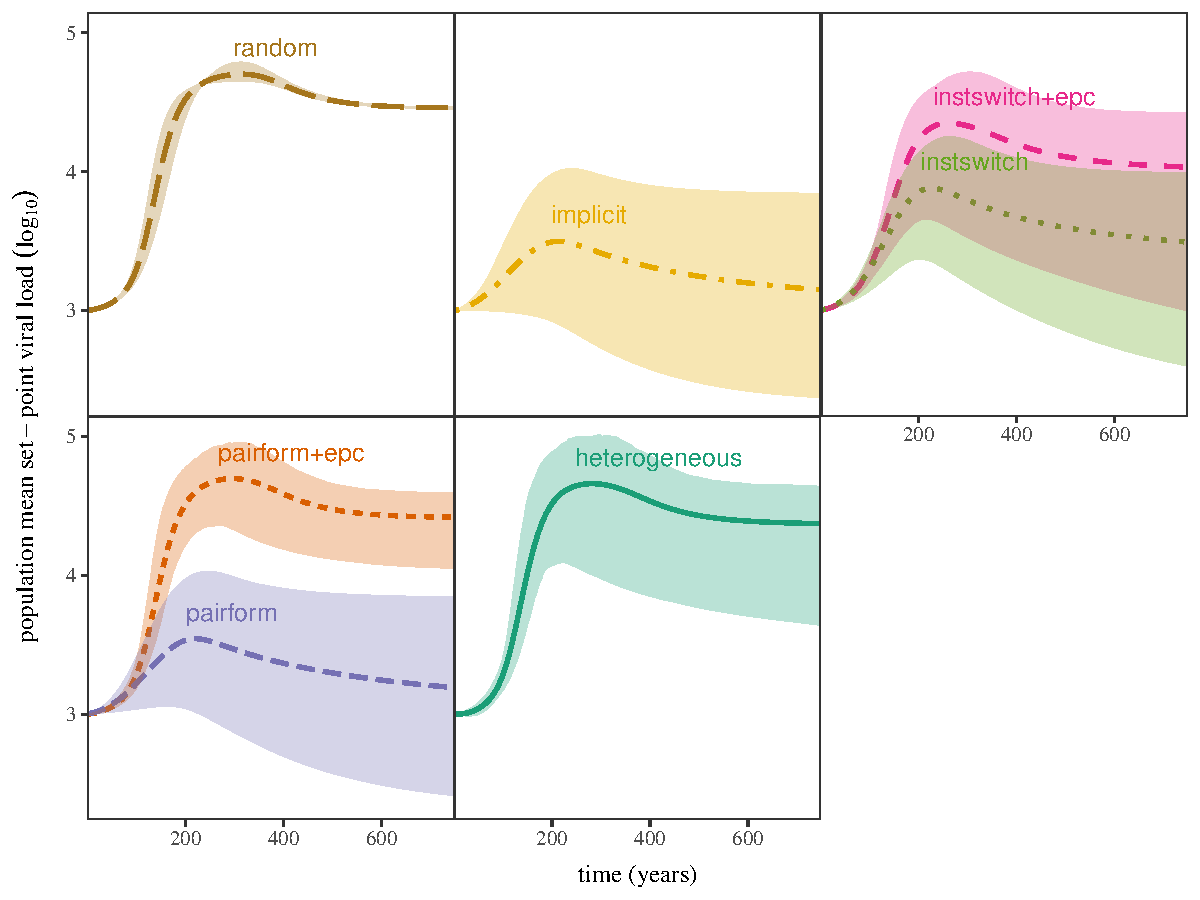
\includegraphics[width=\textwidth]{../figures/fig2.pdf}
\caption{{\bf Envelopes of virulence trajectories under all models.}
All models were run until $t=4000~\textrm{years}$; truncated series are shown here.}
\label{fig:virtraj}
\end{figure}

Our chosen summary statistics (peak time, peak virulence, equilibrium
virulence, and relative peak virulence) all vary considerably across models
\ref{fig:unidist}.
We first consider the models of intermediate realism: implicit,
instantaneous-switching with and without extra-pair contact, and
pair formation without extra-pair contact. Some parameter
sets for these models lead to low equilibrium virulence ($\approx 2.5 \log_{10}$ SPVL);
these same sets lead to correspondingly low
peak virulence ($< 3.5 \log_{10}$ SPVL) and early peak times (before 200 years), 
but high relative peaks ($>1.3$)
(\figurename~\ref{fig:pairplot}, leftmost column) because the equilibrium virulence is low.
At the opposite extreme, parameter sets that produce high equilibrium virulence 
also produce late peaks ($> 200 \text{ years}$), 
high peak virulence, and low relative peaks ($\approx 1.05$).
The pair-formation without extra-pair contact and implicit models
occasionally have parameter sets that select for such low virulence across
the board that they never exceed their initial virulence, leading to a tail
of peak times near zero.

\begin{figure}[!ht]
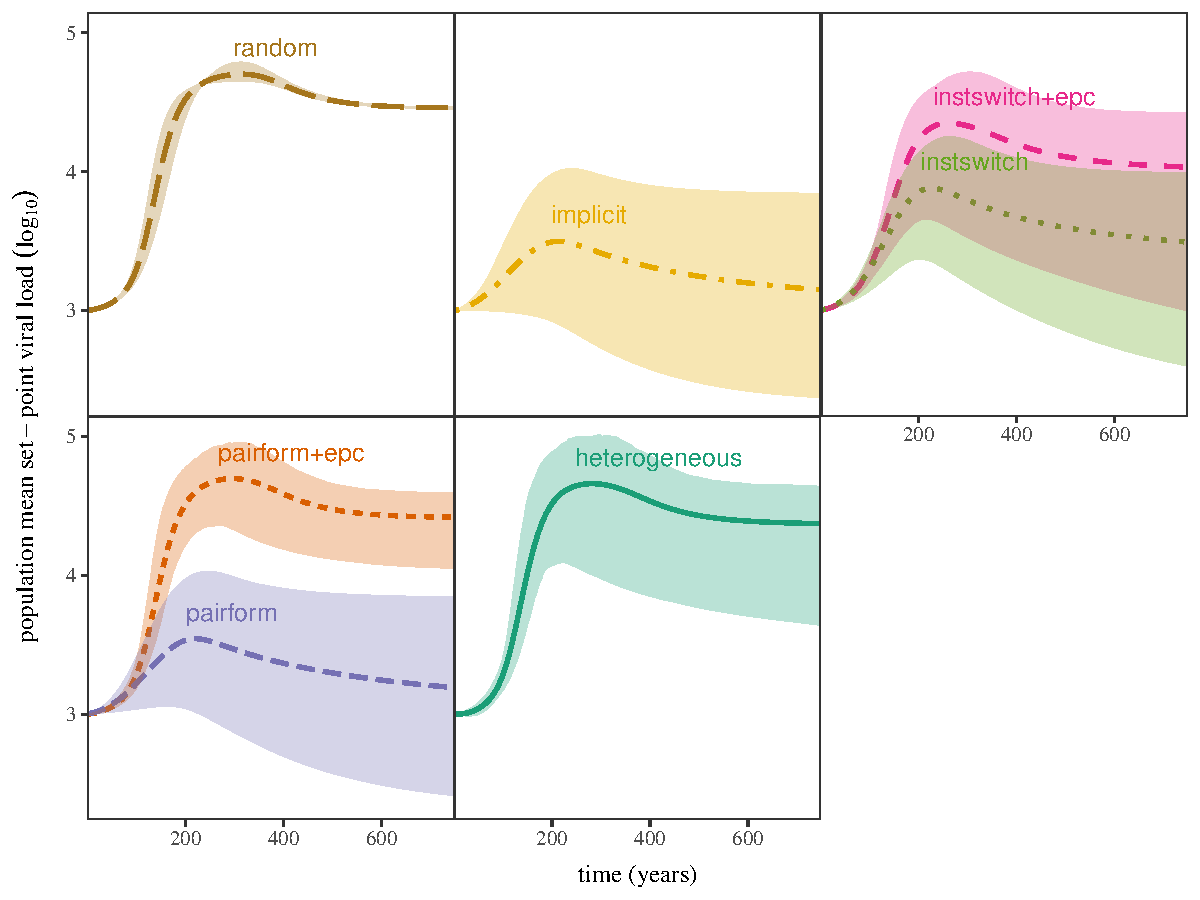
\includegraphics[width=\textwidth]{../figures/fig3.pdf}
\caption{{\bf Univariate distributions of summary statistics.}
The distribution of equilibrium virulence for the random mixing model is very narrow, and has been replaced by a point in order to preserve the vertical axis scaling.}
\label{fig:unidist}
\end{figure}

\begin{figure}[!ht]
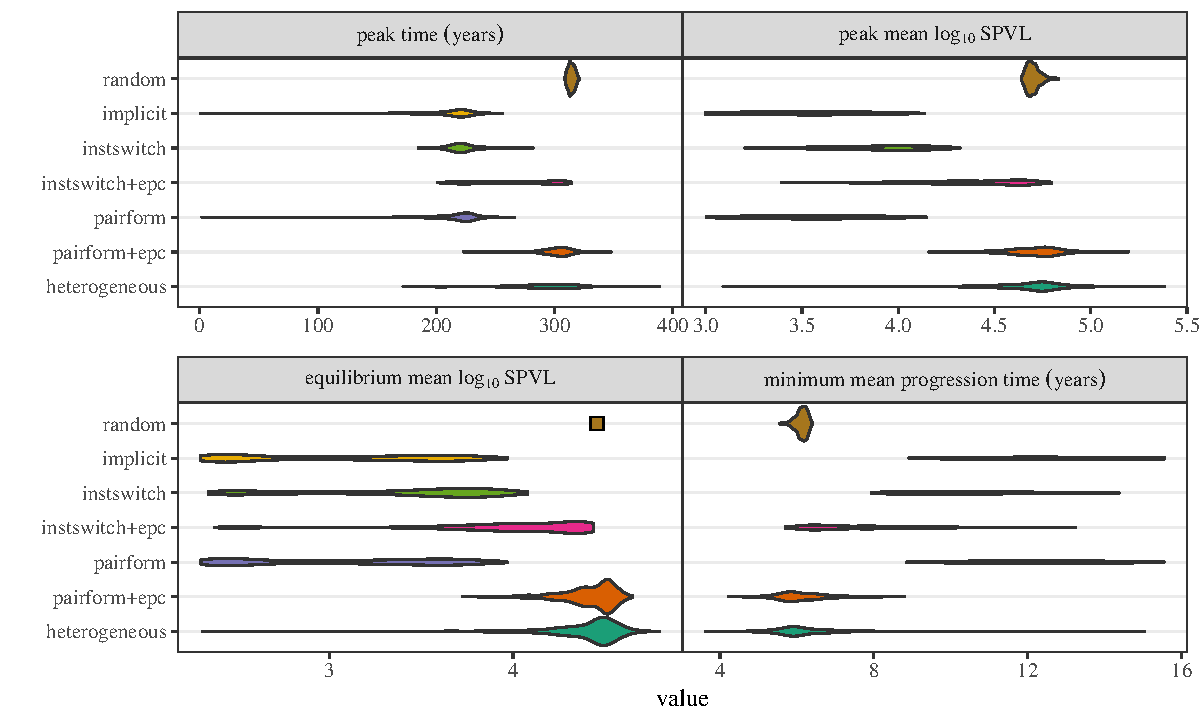
\includegraphics[width=\textwidth]{../figures/fig4.pdf}
\caption{{\bf Pairs plot: bivariate relationships among summary statistics for each model structure.}
Dashed line in equilibrium vs. peak virulence plot shows 1:1 line.}
\label{fig:pairplot}
\end{figure}

The most striking aspect of the univariate comparisons in
\figurename~\ref{fig:unidist}, (and the bivariate comparisons in
\figurename~\ref{fig:pairplot}) is the similarity between the results of the
least (random mixing) and the most complex (pair formation with
extra-pair contact) models. The random-mixing model has lower
variability, because it is unaffected by uncertainty in pair formation
and extra-pair contact parameters, but otherwise the virulence
dynamics of these two extreme models are remarkably similar.
This phenomenon is driven by the strong effects of extra-pair contact in the
model with explicit pair formation and extra-pair contact 
(``pairform+epc'' in \figurename{}s~\ref{fig:virtraj}-\ref{fig:plot_sens}). When individuals spend time uncoupled between
partnerships, and when these single individuals can transmit disease
to coupled individuals, the resulting unstructured mixing overwhelms
the effect of structured mixing within couples, leading to mixing
that is effectively close to random.

Expressing these results in terms of more directly interpretable epidemic
parameters, i.e. using the Hill functions to translate \Lspvl\ to
within-couple transmission probabilities and average time of progression
to AIDS, shows that these differences are practically as well as 
scientifically important. The random-mixing and pairform+epc models
predict minimum times to progression (at the virulence peak) of
5.7 (95\% CI 6.1-6.3) and 6.0 (5.0-7.7) years respectively, while
the implicit model gives progression times about twice as long:
12.5 (9.5-15.6) years. The corresponding differences in 
within-couple transmission
probability are even more extreme, about a fourfold difference:
0.249 (0.24-0.26) and 0.252 (0.19-0.28) per year for the 
random and pairform+epc models vs. 0.059 (0.02-0.13) per year
for the implicit model (Figs~???? show univariate distributions
on the epidemiological scales
of progression time and transmission probability,
for all summary measures and all models).

\begin{figure}[!ht]
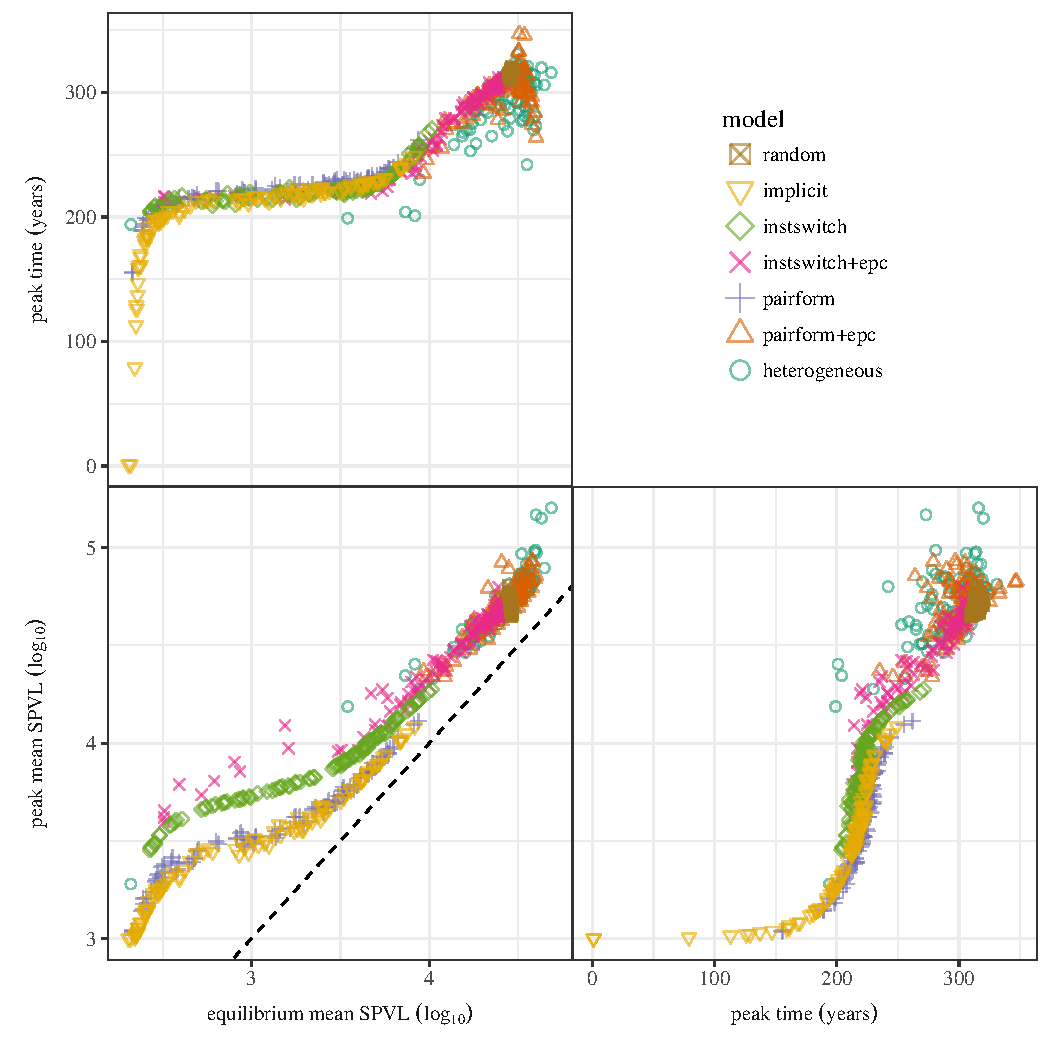
\includegraphics[width=\textwidth]{../figures/fig5.pdf}
\caption{{\bf Sensitivity plot.}
For each parameter in the Latin hypercube sample and each summary statistic, shows the distribution (points) and trend (smooth line) of the summary statistic as a function of the \emph{unscaled} parameter value, i.e. prior to adjusting the parameters to achieve the standard initial epidemic growth rate.}
\label{fig:plot_sens}
\end{figure}

Plotting the bivariate result distributions (\figurename~\ref{fig:pairplot})
shows that most of the summary statistics
are monotonically related, except those involving the relative peak virulence
(bottom row). Changes in parameters that increase the equilibrium
virulence initially increase the peak virulence even more, so
that the relative peak virulence increases as well, but beyond
an equilibrium virulence of about 2.5 \Lspvl\ the peak virulence
increases slower than the equilibrium virulence, leading to a
decrease in the relative peak virulence.

The bivariate relationships also help distinguish the results of 
different models with similar univariate dynamical summaries. While the
relationship between equilibrium virulence and peak time is
similar for all model structures (top left panel), the other
relationships are more separate. In particular, the implicit
and pair-formation (without extra-pair contact) are very similar
to each other, but distinct from the other models. We still do
not have a convincing explanation for this distinction; we
would have expected the implicit model to be most similar to the
the instantaneous-switching model without extra-pair contact,
which most closely matches its derivation. However, we note
that the implicit model derivation is based on defining
the force of infection to match a scaled version of ${\cal R}_0$,
and as such would be expected to match the equilibrium behaviour
but not necessarily the epidemic-phase behaviour of a model
with explicit partnership dynamics.

Finally, the sensitivity plots (\figurename~\ref{fig:plot_sens}) show the effects 
of each parameter on the summary statistics. In almost every case the
effects of the parameters are monotonic; note that
the plot shows the effects of the \emph{unscaled} parameters, i.e.
before they have been calibrated to achieve a standard initial epidemic
growth rate.
Increases in the transmission rates ($\beta_P$, $\beta_D$)
and durations ($D_P$, $D_D$) in the primary and disease stages generally
decrease the equilibrium virulence, peak virulence, and peak time,
although the random and pair-formation+epc 
models have high, relatively
constant values with respect to these parameters. 

The partnership dissolution rate ($c$), which essentially
acts as a contact rate in the model,
increases virulence and peak time in almost all
cases, although the pair-formation+epc
model is again relatively insensitive.
The ratio of extra-pair to within-pair contact ($c_e/c_w$) affects
virulence in the instantaneous-switching+epc model, but not the pair-formation+epc
model (probably because the uncoupled individuals present in the pair-formation+epc
model make extra-pair contact by coupled individuals less important).
Surprisingly, neither of the pair-formation models is particularly sensitive to the 
rate of partnership formation ($\rho$); the rate of uncoupled contact
increases virulence and peak time in the pair-formation+epc model, 
which is the only model to which it applies.

\section*{Discussion}

All models must simplify the world.  Many constraints --- such as data
availability, computation time, or code complexity --- drive the need
for parsimony, with different constraints applying in different
contexts. The critical question that modelers must ask is whether the
simplified model gives adequate answers, or whether the
simplifications lead to qualitative or quantitative errors.
This question is especially important for modelers who
are hoping that their conclusions will guide management decisions.

In the particular example of HIV virulence eco-evolutionary dynamics
and epidemiological, we reach the slightly ironic conclusion that the
effort put into building a more realistic model essentially cancels
out, leaving us in the same position as if we had ignored the problem
of epidemiological complexity entirely and used a naive random-mixing
contact model. In Herbeck \etal's \cite{herbeck_hiv_2014} network model of partnerships, the partnership duration is set to 1 day --- very unrealistic in epidemic terms, but perhaps
actually more true to real-world HIV epidemiological dynamics than a
model with realistic partnership durations that neglects extra-pair
contact \cite{herbeck2016evolution}. Making the model even more realistic
might make the random-mixing model less appropriate. For
example, our model forms partnerships randomly, and assumes that
extra-pair contact is randomly mixing across the population;
one could instead model extra-pair contact as arising from
multiple concurrent partnerships (some, such as contact with sex
workers, of very short duration) and/or more structured partnership
formation (by age, ethnicity, or behaviour group). The effects of
other realistic complications such as explicit modeling of two
sexes (both in contact structure and differential transmission
probabilities), temporal and spatial variation in epidemic processes,
or presence of genetic variation in hosts are harder to predict.

Parameterization is one of the biggest challenges of epidemiological
modeling. In addition to following Champredon \etal\ \cite{champredon_hiv_2013} 
by doing Latin hypercube
sampling across a wide range of epidemiological parameters, we 
calibrated each set of parameters to the same initial epidemic
growth rate, chosen to match the results of previous models
\cite{shirreff_transmission_2011}.  Previous models 
in this area have drawn their
parameters from cohort studies from the 1990s
\cite{wawer2005rates,hollingsworth_hiv1_2008}
rather than doing any explicit calibration to epidemic curves,
but they give reasonable order-of-magnitude
growth rates ($\approx 0.04~\textrm{year}^{-1}$)
for the early stages of the HIV epidemic (although considerably
lower than estimates of $\approx 0.07-0.1~\textrm{year}^{-1}$
based on population genetic reconstructions \cite{faria_early_2014}).
However, our reason for calibrating was not to match any
specific observed epidemic, but rather to make sure that
we were making meaningful comparisons across a range of
models with radically different epidemiological structures, and
hence involving different interpretations of the same quantitative
parameters.  For example, in models with instantaneous switching the
partnership dissolution rate $c$ is identical to the partnership
formation rate; in models with explicit partnership formation,
the partnership formation rate is also $c$ at equilibrium,
but might vary over the course of an epidemic.
It is not obvious whether models with equal parameters but
different structures should be directly compared; calibration
solves this problem.

More generally, any model that wants to be
taken seriously for management and forecasting purposes should
be calibrated to \emph{all} available data, using informative
priors to incorporate both realistic distributions of uncertainty
for all parameters from independent measurements \cite{elderd_uncertainty_2006}
and calibration from population-level observations of epidemic
trajectories. Such a procedure would also be an improvement on the common --- although not universal --- %
practice, which we have followed here,
of assessing uncertainty over uniform ranges rather than
using distributions that allow more continuous variation in support over
the range of a parameter.

Researchers have documented that HIV virulence and set-point viral
load are changing, on time scales comparable to those portrayed here
(e.g., compare \figurename~\ref{fig:virtraj} to Herbeck \etal's
estimated rate of change of 1.3 \Lspvl\ per century [95\% CI -0.1 to
  3] \cite{herbeck_is_2012}), and have begun to build relatively realistic models that
attempt to describe how interventions such as mass antiretroviral
therapy (ART) can be expected to change the trajectory of virulence
evolution \cite{payne_impact_2014,roberts2015impact,herbeck2016evolution}.  While these
efforts are well-intentioned, we caution that epidemiological and
other structural details that are currently omitted from these models
could significantly change their conclusions.

\section*{Acknowledgements}
We would like to thank Christophe Fraser and
David Champredon for access to simulation code;
this work was funded by NSERC Discovery Grant 386590-2010.


\section*{Supporting Information}

% Include only the SI item label in the paragraph heading. Use the \nameref{label} command to cite SI items in the text.
\paragraph*{Appendix S1: model details}
\label{S1_Appendix}

Since we use multi-strain models in which the distribution of \Lspvl\ has been discretized into a vector, we use a matrix notation to describe our models. The five states described in the \emph{Methods} section are replaced with the following notations: $S$, $I_i$, $SS$, $SI_i$, $II_{ij}$, where the subscripts denote the strain with which an individual is infected. For example, $I_i$ is number of infected individuals with \Lspvl\ of $\alpha_i$, and $II_{ij}$ is the number of concordant, HIV-positive couples in which the two partners have \Lspvl\ of $\alpha_i$ and $\alpha_j$ (independent of order; $II_{ij}$ is synonymous with $II_{ji}$). 
Below, we use the Kronecker delta (i.e. $\delta_{ij}=1$ if $i=j$ and 1 otherwise) in a slightly non-standard fashion as an exponent, e.g. $2^{\delta_{ij}}$, to set a value to 2 when $i=j$ and 1 otherwise.

\subsection*{Models 1 (``pairform+epc'') and 2 (``pairform'')}

\subsubsection*{Partnership dynamics}

Single individuals acquire partners at per-person rate $\rho$. Partnership formation rate for $S$, $I_i$ are $\rho S$ and $\rho I_i$, respectively. We follow Champredon \etal's results \cite{champredon_hiv_2013} and assume that single individuals are distributed into coupled states with pair-formation (PF) rates as follows:

\begin{equation}
\begin{aligned}
\PF(SS) &= \frac{\rho S \cdot S}{2 (S + \sum_k I_k)},\\
\PF(SI_i) &= \frac{\rho S \cdot I_i}{S + \sum_k I_k},\\
\PF(II_{ij}) &= \khalf \cdot \frac{\rho I_i \cdot I_j}{S + \sum_k I_k}.
\end{aligned}
\end{equation}

Partnerships dissolve at per-partnership rate $c$: the dissolution rates for $SS$, $SI_i$, and $II_{ij}$ pairs are $c SS$, $c SI_i$, and $c II_{ij}$ respectively. Unlike single strain model, where both individuals leaving the $II$ partnership would enter $I$, we have to account for strains which the individuals in concordant partnership are infected with (i.e. both partners in $II_{ii}$ enter $I_i$ whereas one partner in $II_{ij}$ enters the $I_i$ compartment while the other enters $I_j$). Thus, coupled individuals are distributed into single states through partnership dissolution (DS):

\begin{equation}
\begin{aligned}
\DS(S) &= 2 c SS + \sum_k c SI_k, \\
\DS(I_i) &= c SI_i + \sum_k 2^{\delta_{ik}} c II_{ik}.\\
\end{aligned}
\end{equation}

Combining the partnership formation and dissolution processes yields the following equation:

\begin{equation}
\begin{aligned}
S' &= - \rho S + 2 c SS + \sum_k c SI_k \\
I_i' &= - \rho I_i + c SI_i + \sum_k 2^{\delta_{ik}} c II_{ik}\\
SS' &= \frac{\rho S \cdot S}{2 (S + \sum_k I_k)} - c SS\\
SI_i' &= \frac{\rho S \cdot I_i}{S + \sum_k I_k} - c SI_i\\
II_{ij}' &= \khalf \cdot \frac{\rho I_i \cdot I_j}{S + \sum_k I_k} - c II_{ij}
\end{aligned}
\end{equation}

\subsubsection*{Pair-formation models: infection dynamics}

Within-couple transmission (WT) occurs in both models. An infected partner in $SI$ partnership transmits virus to a susceptible partner at per-partnership rate $\beta$: $\WT(SI_i) = - \beta_i SI_i$. Since we assume that mutation occurs, $II_{ij}$, where $i \neq j$, can be formed from both $SI_i$ and $SI_j$ partnership: $\WT(II_{ij}) = M_{ij} \beta_i SI_i + M_{ji} \beta_j SI_j$. On the other hand, $II_{ii}$ can only be formed from an $SI_i$ partnership: $\WT(II_{ii}) = M_{ii} \beta_i SI_i$. Using the Kronecker delta notation, we obtain the following set of equations that describes within-couple transmission dynamics:

\begin{equation}
\begin{aligned}
\WT(SI_i) &= - \beta_i SI_i,\\
\WT(II_{ij}) &=  \khalf \cdot (M_{ij} \beta_i SI_i + M_{ji}. \beta_j SI_j)
\end{aligned}
\end{equation}

Champredon \etal\ define the proportion of infectious extra-couple and uncoupled contact through the following term:

\begin{equation}
P = \frac{c_u I + c_e (SI + 2 II)}{c_u (S + I) + 2 c_e(SS + SI + II)}.
\end{equation}
The effective uncoupled, $c_u$, and extra couple, $c_e$, contact rates are the product of two terms: uncoupled/extra-couple contact rate $\times$ rate of transmission per contact. Therefore, the transmission rate per contact term in $c_u$ and $c_e$ is canceled out in the equation above. Using this property, we modify the equation above as follows:

\begin{equation}
P = \frac{r_u I + r_e (SI + 2 II)}{r_u (S + I) + 2 r_e(SS + SI + II)},
\end{equation}
where $r_u = c_u/c_w$ and $r_e = c_e/c_w$ are the relative uncoupled/extra-couple contact rates. This simplification is useful in a multi-strain model since we cannot multiply a vector with a single value (e.g. $c_u S$ in denominator) if we use Champredon \etal's equation in its original form. Extending the above equation to multi-strain model so that $P_i$ represents the proportion of the extra-couple and uncoupled contact of an infected individual with strain $i$, we obtain:

\begin{equation}
P_i = \frac{r_u I_i + r_e (SI_i + \sum_k (II_{ik} + \delta_{ik} II_{ik}))}{r_u (S + \sum_k I_k) + r_e(2 SS + \sum_k 2 SI_k + \sum_l \sum_k 2^\delta_{lk} II_{lk} )}.
\end{equation}
Using the equation above, we can model extra-pair transmission (ET). For convenience, uncoupled and extra-couple transmission rates, $c_u$ and $c_e$, will be replaced with $U_i = r_u \beta_i$ and $E_i = r_e \beta_i$ hereafter.

Single susceptible individuals become infected through uncoupled contact at per-person rate $\sum_k P_k U_k$ and enter single infected state. Through mutation, newly infected individuals are distributed into single infected compartments with different strains: $\ET(I_i) = \sum_k M_{ki} P_k U_k S$. Either partner in an $SS$ partnership becomes infected at per-person rate $\sum_k P_k E_k$, and partnership state changes to an $SI$ partnership at the total rate of $\sum_i 2 P_i E_i SS$. The formation of $SI_i$ partnerships is similar to the process through which single susceptible individuals are distributed into single infected compartments: $\ET(SI_i) = \sum_k 2 M_{ki} P_k E_k SS$. Lastly, the susceptible partner in an $SI$ partnership becomes infected from extra-couple contacts at a per-person rate of $\sum_k P_k E_k$, and partnership state changes to an $II$ partnership. As in the previous cases, $SI_i$ partnerships are lost at a rate of $\sum_k P_k E_k SI_i$. The mutation process is similar to that of within-couple transmission. The only difference is that the \Lspvl\ of a newly infected partner is not determined by its social partner but from an extra-couple partner (i.e. the term $P_i$): $\ET(II_{ij}) = (\frac{1}{2})^{\delta_{ij}}(\sum_k (M_{kj} P_k E_k SI_i + M_{ki} P_k E_k SI_j))$. Combining these equations we get the following set of equations that describe all the transmission dynamics:

\begin{equation}
\begin{aligned}
S' =& - \sum_k P_k U_k S,\\
I_i' =& \sum_k M_{ki} P_k U_k S,\\
SS' =&  - \sum_i 2 P_i E_i SS, \\
SI_i' =& \sum_k 2 M_{ki} P_k E_k SS - \beta_i SI_i - \sum_k P_k E_k SI_i,\\
II_{ij}' =& \khalf \cdot (M_{ij} \beta_i SI_i + M_{ji}, \beta_j SI_j) + \khalf \cdot (\sum_k (M_{kj} P_k E_k SI_i\\
&+ M_{ki} P_k E_k SI_j)).
\end{aligned}
\end{equation}

\subsubsection*{Pair formation models: Disease induced mortality}

The per-person disease induced mortality (DM) rate, $\lambda$, is given by taking the reciprocal of the total duration of the infection: $\lambda_i = 1/(D_A + D_P(\alpha_i) + D_D)$. Since we assume an SIS formulation, where infected individuals that die from infection are immediately replaced by an individual in the single susceptible compartment, we obtain the following equation for single infected individuals:

\begin{equation}
\begin{aligned}
\DM(S) &= \sum_k \lambda_k I_k, \\
\DM(I_i) &= - \lambda_i I_i. \\
\end{aligned}
\end{equation}

If an infected individual in a partnership dies, the partnership dissolves. Thus, an $SI_i$ partnership dissolves at per-partnership rate $\lambda_i$, and the susceptible partner enters the single susceptible compartment at rate $\lambda_i SI_i$ (due to the SIS formulation, the infected partner that dies also gives rise, at an equal rate, to an individual entering the single susceptible compartment):

\begin{equation}
\begin{aligned}
\DM(S) &= \sum_k 2 \lambda_k SI_k, \\
\DM(SI_i) &= - \lambda_i SI_i.
\end{aligned}
\end{equation}

Similarly, since $II_{ij}$ partnerships are composed of two infected partners, they dissolve at a per-partnership rate $(\lambda_i + \lambda_j)$. However, two cases, when $i \neq j$ and $i = j$, must be considered separately. When an $II_{ij}$ partnership dissolves due to disease-induced mortality, where $i \neq j$, the death of the partner with strain $i$ causes its partner to enter $I_j$ compartment at rate $\lambda_j II_{ij}$, and vice versa. When an $II_ii$ partnership dissolves, the death of either partner causes the other partner to enter the $I_i$ compartment at rate $\lambda_i II_{ii}$, which sums up to $2\lambda_i II_{ii}$. Combining these dynamics yields:

\begin{equation}
\begin{aligned}
\DM(S) &= \sum_l \sum_k  2^{\delta_{lk}} \lambda_k II_{lk}, \\
\DM(I_i) &=  \sum_k 2^{\delta_{ik}} \lambda_k II_{ik}, \\
\DM(II_{ij}) &= -(\lambda_i + \lambda_j) II_{ij}.
\end{aligned}
\end{equation}

Finally, combining all these equations give us the full model, which is Model 1. We can simply drop the uncoupled and extra-couple transmission terms to obtain equation 2:

\begin{equation}
\begin{aligned}
S' =& - \rho S + 2 c SS + \sum_k c SI_k - \sum_k P_k U_k S + \sum_k \lambda_k I_k \\
&+ \sum_k 2 \lambda_k SI_k + \sum_l \sum_k  2^{\delta_{lk}} \lambda_k II_{lk}\\
I_i' =&  - \rho I_i + c SI_i + \sum_k 2^{\delta_{ik}} c  II_{ik} + \sum_k M_{ki} P_k U_k S- \lambda_i I_i \\
&+ \sum_k 2^{\delta_{ik}} \lambda_k II_{ik} \\
SS' =& \frac{\rho S \cdot S}{2 (S + \sum_k I_k)} - c SS - \sum_i 2 P_i E_i SS \\
SI_i' =& \frac{\rho S \cdot I_i}{S + \sum_k I_k} - c SI_i - \beta_i SI_i + \sum_k 2 M_{ki} P_k E_k SS - \sum_k P_k E_k SI_i   \\
&- \lambda_i SI_i\\
II_{ij}' =& \khalf \cdot \frac{\rho I_i \cdot I_j}{(S + \sum_k I_k)} - c II_{ij} + \khalf \cdot (M_{ij} \beta_i SI_i + M_{ji} \beta_j SI_j) \\
&+ \khalf \cdot (\sum_k (M_{kj} P_k E_k SI_i + M_{ki} P_k E_k SI_j)) -(\lambda_i + \lambda_j) II_{ij}
\end{aligned}
\end{equation}

\subsection*{Models 3 (``instswitch'') and 4 (``instswitch'')}
\subsubsection*{Partnership dynamics}

Since model 3 and 4 assume instantaneous partnership formation, there are only three states: $SS$, $SI_i$, and $II_{ij}$. Partnership dissolution rates are equal to those of model 1 and 2: $\DS(SS) = -cSS$, $\DS(SI_i) = - cSI_i$, and $\DS(II_{ij}) = - c II_{ij}$. Once individuals leave a partnership, they are instantaneously distributed into coupled states. In order to make the equations simpler, we introduce the following two terms: $X$ and $Y_i$, where $X$ denotes the number of susceptible individuals that leave the partnership at a given time, and $Y_i$ the number of infected individuals with \Lspvl\ of $\alpha_i$ who leave partnership at a given time. These temporarily single individuals then form couples through the same partnership formation rule described in the previous section:

\begin{equation}
\begin{aligned}
X &= 2 c SS + \sum_k c SI_k \\
Y_i &= c SI_i + \sum_k 2^{\delta_{ik}} c II_{ik} \\
SS' &= - c SS + \frac{X^2}{2 (X + \sum_k Y_k)}\\
SI_i' &= - c SI_i + \frac{X Y_i}{X + \sum_k Y_k}\\
II_{ij}' &= - c II_{ij} +\khalf \frac{Y_i Y_j}{X + \sum_k Y_k}.
\end{aligned}
\end{equation}

\subsubsection*{Instantaneous-switching models: Infection dynamics}

Model 3 and 4 share the within-couple transmission term with model 1 and 2. Since there is no single (uncoupled) state, only extra-couple transmission exists:

\begin{equation}
P_i = \frac{r_e (SI_i + \sum_k (II_{ik} + \delta_{ik} II_{ik}))}{r_e(2 SS + \sum_k 2 SI_k + \sum_l \sum_k (2^\delta_{kl} II_{lk}) )}.
\end{equation}
Movement from $SS$ state to $SI$ state and $SI$ to $SS$ is modeled through the same equation that is used in model 1 and 2.

\subsubsection*{Instantaneous-switching models: Disease induced mortality}

Disease induced mortality is modeled similar to model 1 and 2. However, as single state does not exist in model 3 and 4, individuals that has left their partnerships due to death of their partners enter temporary compartments and form partners instantly:

\begin{equation}
\begin{aligned}
X &= \sum_k 2 \lambda_k SI_k + \sum_l \sum_k 2^{\delta_{lk}}  \lambda_k II_{lk}, \\
Y_i &=  \sum_k  2^{\delta_{ik}}  \lambda_k II_{ik}, \\
SS' = &= \frac{X^2}{2 (X + \sum_k Y_k)},\\
SI_i' &= - \lambda_i SI_i + \frac{X Y_i}{X + \sum_k Y_k},\\
II_{ij}' &= -(\lambda_i + \lambda_j) II_{ij} + \khalf \cdot \frac{Y_i Y_j}{X + \sum_k Y_k}.
\end{aligned}
\end{equation}

Combining all these dynamics, we have equation 3. If we remove extra-couple transmission, we have equation 4.

\begin{equation}
\begin{aligned}
X =& 2 c SS + \sum_k c SI_k + \sum_k 2 \lambda_k SI_k + \sum_l \sum_k 2^{\delta_{lk}}  \lambda_k II_{lk},\\
Y_i =& c SI_i + \sum_k 2^{\delta_{ik}}  c II_{ik} + \sum_k  2^{\delta_{ik}}  \lambda_k II_{ik}, \\
SS'  =& - c SS + \frac{X^2}{2 (X + \sum_k Y_k)}  - \sum_i 2 P_i E_i SS,\\
SI_i' =& - c SI_i + \frac{X Y_i}{X + \sum_k Y_k} - \beta_i SI_i + \sum_k 2 M_{ki} P_k E_k SS\\
&- \sum_k P_k E_k SI_i - \lambda_i SI_i,\\
II_{ij}'& - c II_{ij} +\khalf \frac{Y_i Y_j}{X + \sum_k Y_k} + \khalf \cdot (M_{ij} \beta_i SI_i + M_{ji} \beta_j SI_j)\\
&+ \khalf \cdot (\sum_k (M_{kj} P_k E_k SI_i + M_{ki} P_k E_k SI_j)) -(\lambda_i + \lambda_j) II_{ij}.
\end{aligned}
\end{equation}

\subsection*{Implicit model}

Following \cite{shirreff_transmission_2011}, Model 5 is an implicit instantaneous partnership formation model that uses an adjusted transmission rate, $\beta^\ast$, that is derived from \cite{hollingsworth_hiv1_2008}'s approximate basic reproduction number:

\begin{equation}
\beta^\ast_i = \frac{c \beta_i}{c + \beta_i + \lambda_i}.
\end{equation}
Thus, we get the following model:

\begin{equation}
\begin{aligned}
S' & = \sum_k \lambda_k I_k - \sum_k \beta^\ast_k S I_k.\\
I_i' & = \sum_k M_{ki} \beta^\ast_k S I_k - \lambda_i I_i.
\end{aligned}
\end{equation}

\subsection*{Random-mixing model}

Model 6 is a random mixing model. It is modeled in a same way as model 5 without the adjusted transmission rate:

\begin{equation}
\begin{aligned}
S' & = \sum_k \lambda_k I_k - \sum_k \beta_k S I_k,\\
I_i' & = \sum_k M_{ki} \beta_k S I_k - \lambda_i I_i.
\end{aligned}
\end{equation}

\subsection*{Heteregenous model}

We extend "pairform+epc model" by allowing for heterogeneity in sexual behaviour. Since pairform+epc model captures four distinct sexual behaviours -- pair formation, pair dissolution, extra-couple mixing, and uncoupled mixing -- we assume that all four parameters that model the mentioned behaviours are scaled by the same factor based on the risk group. In other words, an individual in a higher risk is more likely to form a stable partnership, leave a stable partnership, and engage in a extra-couple/uncoupled mixing. We denote this scaling parameter as $\varphi_i$ where $i$ is the risk group. For simplicity, we assume that the transmission rate per partnership is not affected by sexual behaviour.

\subsubsection*{Partnership dynamics}

Individuals in a risk group $i$ leave single state at per-person rate $\varphi_i \rho$. Let $XY_{ij,kl}$ be a coupled state where $X$ and $Y$ are the infection status (susceptible or infected) of each partner, $k$ and $l$ are the risk groups $X$ and $Y$ belong to respectively, and $i$ and $j$ are the strains of an infected partner. If a partner is susceptible, strain index is replaced by $\cdot$. For example, $SI_{\cdot j,kl}$ is the number of partners where the susceptible partner is in risk group $k$ and infected partner is in risk group $l$ and has \Lspvl\ of $\alpha_j$. For simplicity, we assume that people mix randomly. Then, we can write the partnership formation process as follows:

\begin{equation}
\PF(XY_{ij, kl}) = \kkhalf \frac{\varphi_k \rho X_{i,k} \varphi_l \rho Y_{j, l}}{\sum\limits_m \varphi_m \rho (S_{\cdot, m} + \sum\limits_n I_{n,m})}
\end{equation}

For dissolution process, individual in risk group $i$ expects to leave partnership at a rate $\varphi_i c$. If partnership is formed between two individuals from a different risk group, rate at which they leave the partnership differs. We resolve this conflict by assuming that a partnership dissolution rate of a couple is equal to the average of that of two partners. Therefore, $XY_{ij, kl}$ dissolve at per-partnership rate $\frac{\varphi_k + \varphi_l}{2} c$, and both $X_{i,k}$ and $Y_{j,l}$ partners return to single state at the same rate.

\subsubsection*{Heterogeneous models: Infection dynamics}

Since we assume that the rate of transmission per partnership stays constant across different risk groups, within-couple infection process is similar to other models:

\begin{equation}
\begin{aligned}
WT(SI_{\cdot j, kl} &= - \beta_j SI_{\cdot j, kl}\\
WT(II_{ij, kl}) &= \kkhalf \cdot (M_{ji} \beta_j SI_{\cdot j, kl} + M_{ij} \beta_i SI_{\cdot i, lk})
\end{aligned}
\end{equation}

Note that $II_{ij,kl}$ can be formed from two types of partnerships: 1) Infected partner with \Lspvl\ of $\alpha_j$ and risk group of $l$ infects a susceptible partner in risk group $k$, yielding \Lspvl\ of $\alpha_i$ through mutation. 2) Infected partner with \Lspvl\ of $\alpha_i$ and risk group of $k$ infected a susceptible partner in risk group $l$, yielding \Lspvl\ of $\alpha_j$ through mutation. On the other hand, if $i = j$ and $k = l$, $II_{ii,kk}$ can only be formed from $SI_{\cdot i, kk}$ partnership, which is resolved by $\kkhalf$.

Heterogeneous extra-couple and uncoupled contact process is similar to partnership formation process. Relative uncoupled/extra-couple contact rates are scaled by the factor of $\varphi_i$, where $i$ is the risk group. First, we define $Q_{i}$ as the total rate of uncoupled/extra couple contact by individuals in risk group $k$:

\begin{equation}
\begin{aligned}
Q_i = &\varphi_i r_u (S_{\cdot,i} +  \sum_j I_{j,i}) + \varphi_i r_e \bigg( \sum_k 2^{\delta_{ik}} SS_{\cdot, ik} +\\
&\sum_l \sum_j (SI_{\cdot j,il} + SI_{\cdot j, li}) + \sum_j \sum_l \sum_k 2^{\delta_{kl} \delta_{ij}} II_{kl,ij} \bigg)
\end{aligned}
\end{equation}
We now define $P_{k,i}$ as the proportion of the extra-couple and uncoupled contact that arises from an infected individual from risk group $i$ with \Lspvl\ of $\alpha_k$:
\begin{equation}
P_{k,i} = \frac{\varphi_i r_u I_{k,i} + \varphi_i r_e (SI_{k,i} + \sum_j \sum_l 2^{\delta_{kl} \delta_{ij} } II_{kl,ij} )}{\sum_j Q_j}
\end{equation}
Since the relative uncoupled/extra couple contact ratio are scaled by the factor of $\varphi_i$, uncoupled and extra-couple transmission rates are scaled by the same factor as well: $U_{k,i} = \varphi_i r_u \beta_k$ and $E_{k,i} = \varphi_i r_e \beta_k$. Once again, we assume random mixing between individuals. Then, a susceptible individual in risk group $i$ becomes infected through extra-couple and uncoupled contact at a per capita rate of $\sum_j \sum_k P_{k,j} X_{k,i}$. Once infected, individuals are distributed into each Strain categories through mutation.

\subsubsection*{Heterogeneous model: Disease induced mortality}

Disease induced mortality is not affected by the sexual behaviour of an individual. 

\subsection*{Initial distribution of infected individuals}

We follow Champredon \etal's result to calculate the initial distribution of infected individuals. For model 1 and 2, we have disease equilibrium state of $S^* = \frac{c}{c + \rho}$ and $SS^* = \frac{1-S^*}{2}$. We let $\epsilon = 10^{-4}$, which is the total number of infected individuals in the beginning of simulation and $D$ be the vector such that $D_i$ represent the proportion of individuals with \Lspvl\ of $i$. $Y_i$ is taken from normal distribution with mean 3 and is normalized so that $\sum_i D_i = 1$. Then, we have the following initial distribution of each states:

\begin{equation}
\begin{aligned}
S(0) &= (1 - \epsilon) S^*, \\
SS(0) &= (1 - \epsilon)^2 SS^*,\\
SI_i(0) &= 2 \epsilon (1-\epsilon) SS^* D_i,\\
I_i(0) &=  \epsilon S^* D_i,\\
II_{ij}(0) &=  \khalf 2\epsilon^2 SS^* D_i D_j.
\end{aligned}
\end{equation}
Since model 3 and 4 do not have single state, $SS^*=1$ at the disease free equilibrium and the initial distribution becomes as follows:

\begin{equation}
\begin{aligned}
SS(0) &= (1 - \epsilon)^2 SS^*,\\
SI_i(0) &= 2 \epsilon (1-\epsilon) SS^* D_i,\\
II_{ij}(0) &=  \khalf 2\epsilon^2 SS^* D_i D_j.
\end{aligned}
\end{equation}
As model 5 is an implicit model, which does not consider different stages of partnership, we have the following initial distribution:

\begin{equation}
\begin{aligned}
S(0) &= 1 - \epsilon,\\
I_i(0) &=  \epsilon D_i.
\end{aligned}
\end{equation}
Model 6 has the same distribution of initial infected individuals as model 5.

Lastly, for heterogeneity model, we assume that the risk distribution of the population follows gamma distribution and calculate the shape and scale parameters given the mean and squared coefficient of variation. Using the shape and scale parameterws, we define gamma quantile function $Q(p)$ and $p_j =  \tsub{p}{min} + (\tsub{p}{max} - \tsub{p}{min}) \frac{j-1}{n_r + 1}$, where $n_r$ is number of risk groups and $j = 1, 2, 3, \dots, n_r + 1$. Since $Q(1) = \infty$, we set $\tsub{p}{max} = 0.99$ and $\tsub{p}{min} = 0.01$. Then, we define $\varphi_i = \frac{Q(p_j) + Q(p_{j+1})}{2}$. We define $R_i$ as the proportion of individuals in risk group $i$ in a disease free equilibrium and assume $R_i$ is equal for all $i$, i.e. $R_i = \frac{1}{n_r}$. In order to start the simulation in a quasi-equilibrium state, we first run the model with the following initial state:

\begin{equation}
\begin{aligned}
S_{\cdot,i}(0) &= (1 - \epsilon) R_i,\\
I_{k,i}(0) &= \epsilon D_k R_i,\\
SS_{\cdot,ij}(0) &= SI_{\cdot k, ij}(0) = II_{kl,ij} (0) = 0.\\
\end{aligned}
\end{equation}
For this particular simulation, we disregard infection process as well as disease induced mortality in order to preserve the strain distribution of infected individuals. Furthermore, since the scaling parameter, $\gamma$, does not affect the risk group distribution in the absence of disease transmission, we increase the scaling parameter to 5 ($\gamma = 5$) to speed up the simulation and run the model for 50 years. After the model has reached its quasi-equilibrium state, we take this distribution of susceptible and infected individuals as the initial state of the actual simulation.

\paragraph*{Appendix S2: dynamics of transmission and virulence}

\label{S2_Appendix}

This section presents

\begin{figure}[!ht]
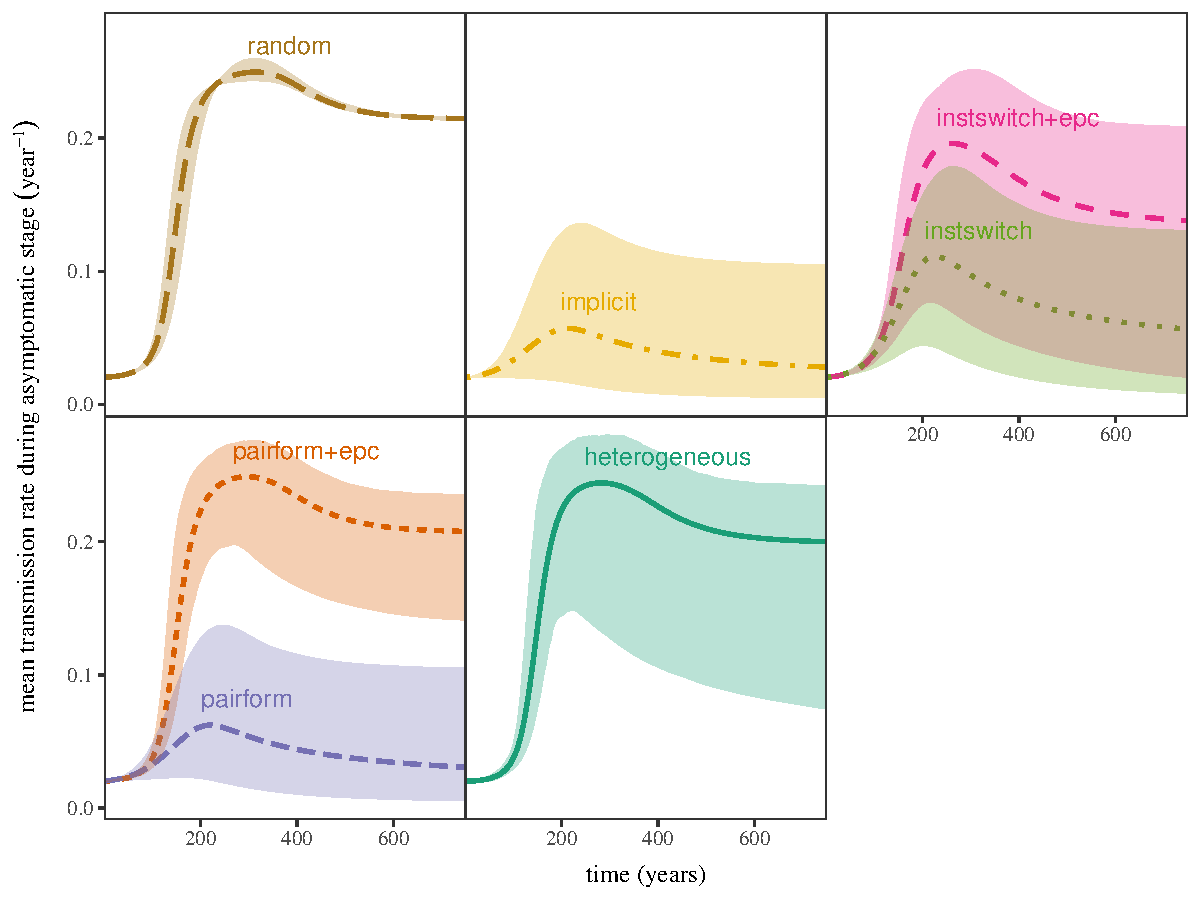
\includegraphics[width=\textwidth]{../figures/fig_S2_1.pdf}
\caption{{\bf Envelopes of transmission trajectories under all models.}
This figure matches \figurename~\ref{fig:virtraj}, but displays the
envelope of population-mean transmission probabilities rather than \Lspvl\ over time
for each model.
}
\label{fig:transtraj}
\end{figure}

\begin{figure}[!ht]
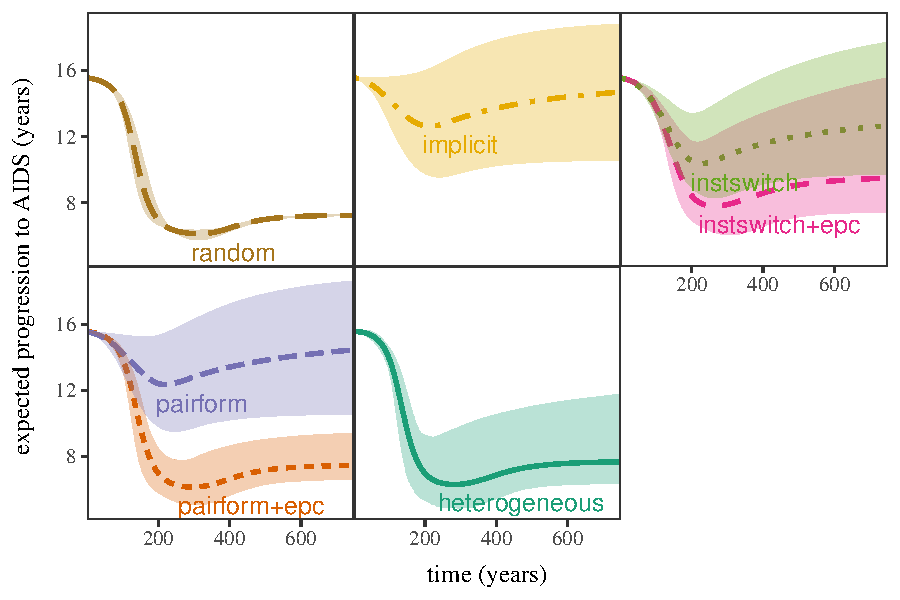
\includegraphics[width=\textwidth]{../figures/fig_S2_2.pdf}
\caption{{\bf Envelopes of progression trajectories under all models.}
This figure matches \figurename~\ref{fig:virtraj}, but displays the
envelope of population-mean expected time of progression to AIDS (i.e., length of
intermediate HIV phase) rather than \Lspvl\ over time
for each model.
}
\label{fig:durtraj}
\end{figure}

\begin{figure}[!ht]
  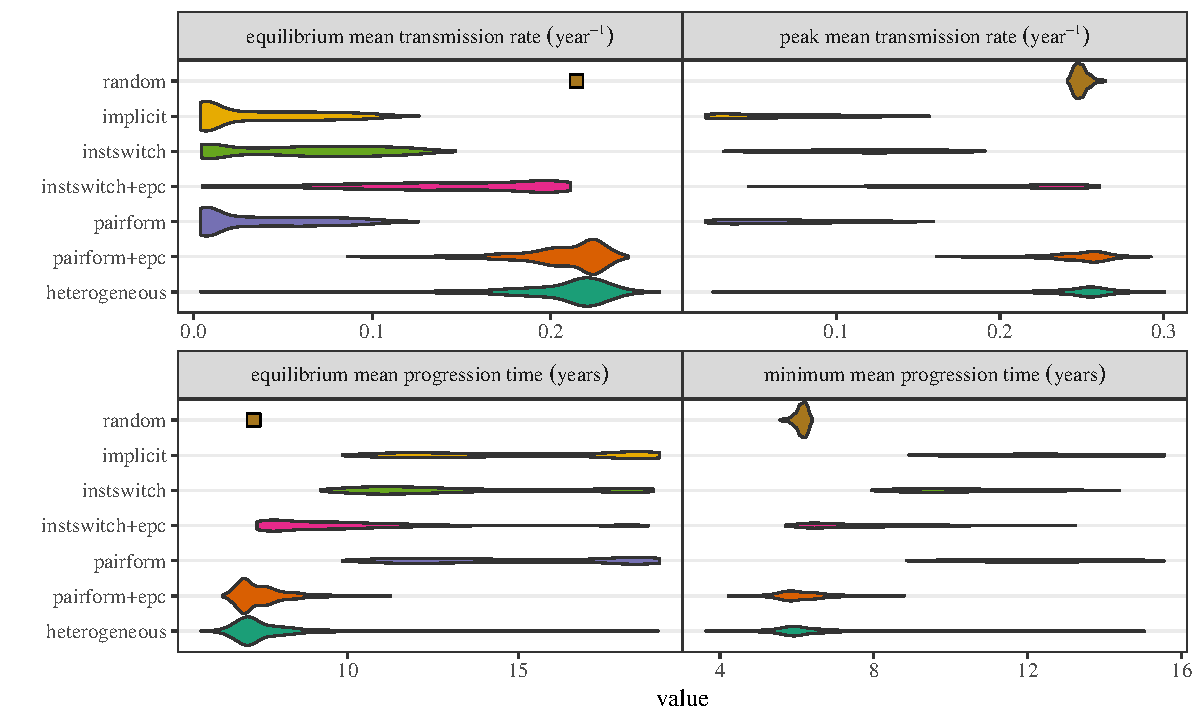
\includegraphics[width=\textwidth]{../figures/fig_S2_3.pdf}
\caption{{\bf Univariate distributions of transmission probabilities and progression.}
This figure matches \figurename~\ref{fig:unidist}, but displays the
univariate distributions for the transmission probability and 
progression time at the virulence
peak and at the epidemiological equilibrium,
rather than the distributions of \Lspvl.
}
\label{fig:tranprogsum}
\end{figure}

\nolinenumbers

% Either type in your references using
% \begin{thebibliography}{}
% \bibitem{}
% Text
% \end{thebibliography}
%
% or
%
% Compile your BiBTeX database using our plos2015.bst
% style file and paste the contents of your .bbl file
% here.
% 

% \bibliography{virulence}
\begin{thebibliography}{10}

\bibitem{Ebert1999}
Ebert D.
\newblock The evolution and expression of parasite virulence.
\newblock In: Stearns SC, editor. Evolution in Health \& Disease. New York:
  Oxford University Press, Oxford, UK; 1999. p. 161--172.

\bibitem{EbertBull2003}
Ebert D, Bull JJ.
\newblock Challenging the trade-off model for the evolution of virulence: is
  virulence management feasible?
\newblock Trends Microbiol. 2003;11(1):15--20.

\bibitem{alizon_adaptive_2015}
Alizon S, Michalakis Y.
\newblock Adaptive virulence evolution: the good old fitness-based approach.
\newblock Trends in Ecology \& Evolution. 2015;30(5):248--254.
\newblock doi:{10.1016/j.tree.2015.02.009}.

\bibitem{Dwyer+1990}
Dwyer G, Levin SA, Buttel L.
\newblock A simulation model of the population dynamics and evolution of
  myxomatosis.
\newblock Ecol Monog. 1990;60:423--447.

\bibitem{mackinnon1999genetic}
Mackinnon MJ, Read AF.
\newblock Genetic relationships between parasite virulence and transmission in
  the rodent malaria {{\em Plasmodium chabaudi}}.
\newblock Evolution. 1999; p. 689--703.

\bibitem{jensen2006empirical}
Jensen KH, Little T, Skorping A, Ebert D.
\newblock Empirical support for optimal virulence in a castrating parasite.
\newblock PLoS Biol. 2006;4(7):e197.

\bibitem{deroode2008virulence}
De~Roode JC, Yates AJ, Altizer S.
\newblock Virulence-transmission trade-offs and population divergence in
  virulence in a naturally occurring butterfly parasite.
\newblock Proceedings of the National Academy of Sciences.
  2008;105(21):7489--7494.

\bibitem{Fraser+2007}
Fraser C, Hollingsworth TD, Chapman R, de~Wolf F, Hanage WP.
\newblock Variation in {HIV}-1 set-point viral load: Epidemiological analysis
  and an evolutionary hypothesis.
\newblock PNAS. 2007;104:17441--17446.

\bibitem{fraser_virulence_2014}
Fraser C, Lythgoe K, Leventhal GE, Shirreff G, Hollingsworth TD, Alizon S,
  et~al.
\newblock Virulence and Pathogenesis of {HIV}-1 Infection: An Evolutionary
  Perspective.
\newblock Science. 2014;343(6177):1243727.
\newblock doi:{10.1126/science.1243727}.

\bibitem{shirreff_transmission_2011}
Shirreff G, Pellis L, Laeyendecker O, Fraser C.
\newblock Transmission Selects for {HIV-1} Strains of Intermediate Virulence: A
  Modelling Approach.
\newblock PLoS Computational Biology. 2011;7(10):e1002185.
\newblock doi:{10.1371/journal.pcbi.1002185}.

\bibitem{herbeck_hiv_2014}
Herbeck JT, Mittler JE, Gottlieb GS, Mullins JI.
\newblock An {HIV} Epidemic Model Based on Viral Load Dynamics: Value in
  Assessing Empirical Trends in {HIV} Virulence and Community Viral Load.
\newblock {PLoS} Comput Biol. 2014;10(6):e1003673.

\bibitem{day_virulence_2004}
Day T, Proulx SR.
\newblock A General Theory for the Evolutionary Dynamics of Virulence.
\newblock The American Naturalist. 2004;163(4):E40--E63.
\newblock doi:{10.1086/382548}.

\bibitem{alizon_price_2009}
Alizon S.
\newblock The {Price} equation framework to study disease within-host
  evolution.
\newblock Journal of Evolutionary Biology. 2009;22(5):1123--1132.
\newblock doi:{10.1111/j.1420-9101.2009.01726.x}.

\bibitem{champredon_hiv_2013}
Champredon D, Bellan S, Dushoff J.
\newblock {HIV} Sexual Transmission Is Predominantly Driven by Single
  Individuals Rather than Discordant Couples: A Model-Based Approach.
\newblock PLoS ONE. 2013;8(12):e82906.
\newblock doi:{10.1371/journal.pone.0082906}.

\bibitem{hollingsworth_hiv1_2008}
Hollingsworth TD, Anderson RM, Fraser C.
\newblock {HIV}-1 Transmission, by Stage of Infection.
\newblock Journal of Infectious Diseases. 2008;198(5):687--693.
\newblock doi:{10.1086/590501}.

\bibitem{blower_drugs_1991}
Blower SM, Hartel D, Dowlatabadi H, Anderson RM, May RM.
\newblock Drugs, Sex and {HIV}: A Mathematical Model for {New York City}.
\newblock Philosophical Transactions of the Royal Society of London B:
  Biological Sciences. 1991;331(1260):171--187.
\newblock doi:{10.1098/rstb.1991.0006}.

\bibitem{ma_estimating_2014}
Ma J, Dushoff J, Bolker BM, Earn DJD.
\newblock Estimating Initial Epidemic Growth Rates.
\newblock Bulletin of Mathematical Biology. 2014;76(1):245--260.
\newblock doi:{10.1007/s11538-013-9918-2}.

\bibitem{wallinga_how_2007}
Wallinga J, Lipsitch M.
\newblock How generation intervals shape the relationship between growth rates
  and reproductive numbers.
\newblock Proceedings of the Royal Society of London B: Biological Sciences.
  2007;274(1609):599--604.
\newblock doi:{10.1098/rspb.2006.3754}.

\bibitem{soetaert_solving_2010}
Soetaert K, Petzoldt T, Setzer RW.
\newblock Solving Differential Equations in {R}: Package {deSolve}.
\newblock Journal of Statistical Software. 2010;33(9):1--25.
\newblock doi:{10.18637/jss.v033.i09}.

\bibitem{herbeck2016evolution}
Herbeck J, Mittler J, Gottlieb G, Goodreau S, Murphy J, Cori A, et~al.
\newblock Evolution of {HIV} virulence in response to widespread scale up of
  antiretroviral therapy: a modeling study.
\newblock bioRxiv. 2016; p. 039560.

\bibitem{wawer2005rates}
Wawer MJ, Gray RH, Sewankambo NK, Serwadda D, Li X, Laeyendecker O, et~al.
\newblock Rates of {HIV}-1 transmission per coital act, by stage of {HIV}-1
  infection, in {Rakai}, {Uganda}.
\newblock Journal of Infectious Diseases. 2005;191(9):1403--1409.

\bibitem{faria_early_2014}
Faria NR, Rambaut A, Suchard MA, Baele G, Bedford T, Ward MJ, et~al.
\newblock The early spread and epidemic ignition of {HIV}-1 in human
  populations.
\newblock Science (New York, NY). 2014;346(6205):56--61.
\newblock doi:{10.1126/science.1256739}.

\bibitem{elderd_uncertainty_2006}
Elderd BD, Dukic VM, Dwyer G.
\newblock Uncertainty in predictions of disease spread and public health
  responses to bioterrorism and emerging diseases.
\newblock Proceedings of the National Academy of Sciences. 2006;103(42):15693
  --15697.
\newblock doi:{10.1073/pnas.0600816103}.

\bibitem{herbeck_is_2012}
Herbeck JT, Müller V, Maust BS, Ledergerber B, Torti C, Di~Giambenedetto S,
  et~al.
\newblock Is the virulence of {HIV} changing? {A} meta-analysis of trends in
  prognostic markers of {HIV} disease progression and transmission.
\newblock AIDS (London, England). 2012;26(2):193--205.
\newblock doi:{10.1097/QAD.0b013e32834db418}.

\bibitem{payne_impact_2014}
Payne R, Muenchhoff M, Mann J, Roberts HE, Matthews P, Adland E, et~al.
\newblock Impact of {HLA}-driven {HIV} adaptation on virulence in populations
  of high {HIV} seroprevalence.
\newblock Proceedings of the National Academy of Sciences.
  2014;111(50):E5393--E5400.
\newblock doi:{10.1073/pnas.1413339111}.

\bibitem{roberts2015impact}
Roberts HE, Goulder PJ, McLean AR.
\newblock The impact of antiretroviral therapy on population-level virulence
  evolution of {HIV}-1.
\newblock Journal of The Royal Society Interface. 2015;12(113):20150888.

\end{thebibliography}


\end{document}

